\documentclass[tog]{acmsiggraph}

\usepackage{tabularx}

\renewcommand{\arraystretch}{1.2}



\title{Simulating evolutions of castles \\ \textit{Battles python module usage}}

\author{Albert Mas}
\pdfauthor{Albert Mas}

\keywords{}

\begin{document}
 
\maketitle
 

 
\section{Introduction}

To run a city evolution simulation, just instantiate a \texttt{Run} object and execute it:

\begin{verbatim}
  from Battles.Run import Run 
 
  r = Run(playdataxml = "simulation.xml",
          setttingsxml = "settings.xml")
  r.Execute()
\end{verbatim} 

The \texttt{playdataxml} parameter is the XML file with the simulation set of parameters. 
The \texttt{settingsxml} parameter is the XML file with the global application parameters, and it is optional. 
If it is not specified, it uses the default one: \texttt{Battles/Utils/settings.xlm}.

There are two play modes: city evolution and battle simulation.
The city evolution simulates the city growth and allow to simulate battles.
The battle simulation mode only simulates a battle.
On the next sections the XML specifications of each file will be explained.



\section{Simulation XML: City evolution}

The simulation XML file contains the paramters to define a city evolution. 
It is wrapped by \texttt{<Game></Game>} tag, and the elements that must contain are specified in the next table. 
All parameters are mandatory, except those ones that are marked as optional.


\begin{tabularx}{0.48\textwidth}{ |l|X| }
\hline 
\textbf{Parameter} & \textbf{Description} \\[0.15cm]
\hline
\texttt{Type} & Type of simulation\\
 & Available values: \\
 & \\
 & \quad\texttt{CityExpansion}: Standard simulation \\
 & \quad\texttt{Battle}: See Section \ref{sec:battle} \\
 & \\
 \hline 
 \texttt{TimeRange} & Simulation time range, in centuries. \\
 & Format example: \\
 & \\
 & \quad\texttt{[8, 19]} \\
 & \\
 \hline
 \texttt{Battlefield} & Battlefield data. See Section \ref{sec:battlefield} \\
 \hline
 \texttt{Castle} & Castle data. See Section \ref{sec:castle} \\
 \hline
 \texttt{CityEvolutions} & City evolution patterns. See Section \ref{sec:cityevolutions} \\
 \hline
 \texttt{CityExpansion} & City expansion dates. See Section \ref{sec:cityexpansion} \\
 \hline
 \texttt{BattleEvents} & See Section \ref{sec:battleevents} \\
 \hline
 \texttt{ExpansionCheckings} & Checkin dates. See Section \ref{sec:expansioncheckings}\\
 \hline
 \texttt{StarFortress} & Starfortreess creation data. See Section \ref{sec:starfortress} \\
 \hline
\end{tabularx} 




You must take into account the next issues:

\begin{itemize}
 \item There are not any restriction on scale or units, althought is recommended to use meters. You must use the same scale/units for all properties.
 \item Use decimal values for all measures.
 \item The main view is a 2D plane view of the castle and the battlefield. The view coordinate systen starts at the top left corner window.
\end{itemize}







\subsection{Battlefield}
\label{sec:battlefield}

This element defines the battlefield parameters. 
The battlefield is just the 2D plane where the simulation runs.


\begin{tabularx}{0.48\textwidth}{ |l|X| }
\hline 
\textbf{Parameter} & \textbf{Description} \\[0.15cm]
 \hline
 \texttt{Bounding} & Battlefield size. The battlefield is a square.\\
 & The value is the square side length\\
 \hline
 \texttt{CellSize} & Size of battlefield squares subdivision. The battlefield cell contains only one battalion. Therefore, the cell size defines also the battalion maximum size. Recommended value is 10.0.\\
 \hline
 \texttt{Rivers} & Rivers definition. Rivers are defined by a list of polylines with width. Each polyline is defined as follows on the next example: \\
 & \\
 & \quad\texttt{<Trace>} \\
 & \quad\quad\texttt{<Width>30.0</Width>}\\
 & \quad\quad\texttt{<Polyline>}\\
 & \quad\quad\quad\texttt{<Vertex>}\\
 & \quad\quad\quad\quad\texttt{[28.2, 94.7]}\\
 & \quad\quad\quad\texttt{</Vertex>}\\
 & \quad\quad\quad\texttt{...}\\
 & \quad\quad\quad\texttt{<Vertex>}\\
 & \quad\quad\quad\quad\texttt{[52.6, 92.8]}\\
 & \quad\quad\quad\texttt{</Vertex>}\\
 & \quad\quad\texttt{</Polyline>}\\
 & \quad\texttt{</Trace>}\\
 & \\
 \hline
\end{tabularx} 




 
\subsection{Castle}
\label{sec:castle}

This element defines the castle initial shape.

\begin{tabularx}{0.48\textwidth}{ |l|X| }
\hline 
\textbf{Parameter} & \textbf{Description} \\[0.15cm]
 \hline
  \texttt{Orientation} & Castle front direction. It is used as reference to construct well oriented squared towers. \\
  & The value is a 2D vector. Format example:  \\ 
   & \\
  & \quad\texttt{[0.0, -1.0]}\\
  & \\
  & (see Figure \ref{fig:cityevolution_castle}).\\
 \hline
\end{tabularx}  
 
\begin{tabularx}{0.48\textwidth}{ |l|X| }
\hline 
\textbf{Parameter} & \textbf{Description} \\[0.15cm]
 \hline
 \texttt{OldCity} & Initial castle shape defined by a list of initial inner houses. The curtain wall will be constructed wrapping around these houses. \\
 & Format example for each house:\\
 & \\
 & \quad\texttt{<House>}\\
 & \quad\quad\texttt{[100.0, 250.0]}\\
 & \quad\texttt{</House>}\\
  & \\
 & , where each value is the house 2D center point (see Figure \ref{fig:cityevolution_castle}).\\
 \hline
 \texttt{Moat} & If is specified, the castle has a wrapping moat. The tag must has the \texttt{<HasWater>} tag that defines if moat has water or not.\\
 \hline
 \texttt{Shape} & Initial castle shape defined by a polyline from a list of vertices, where each vertex is defined by \texttt{Vertex} tag. Each vertex has the 2D position and the kind of tower. Format example:\\
 & \\
 & \quad\texttt{<Vertex>}\\
 & \quad\quad\texttt{<Point>}\\
 & \quad\quad\quad\texttt{[970.0, 1125.0]}\\
 & \quad\quad\texttt{</Point>}\\
 & \quad\quad\texttt{<TowerType>}\\
 & \quad\quad\quad\texttt{SquaredTower}\\
 & \quad\quad\texttt{</TowerType>}\\
 & \quad\texttt{</Vertex>}\\
 & \\
 & The tower type values are: \texttt{SquaredTower}, \texttt{RoundedTower} or \texttt{Tower} if a random choice is desired (the random choice is a fuzzy selection from current year simulation over the towers timerange table shown in Section \ref{sec:settingscastletower}. The tower type is optional.\\
 \hline
\end{tabularx} 


\begin{figure}[ht]
  \centering
  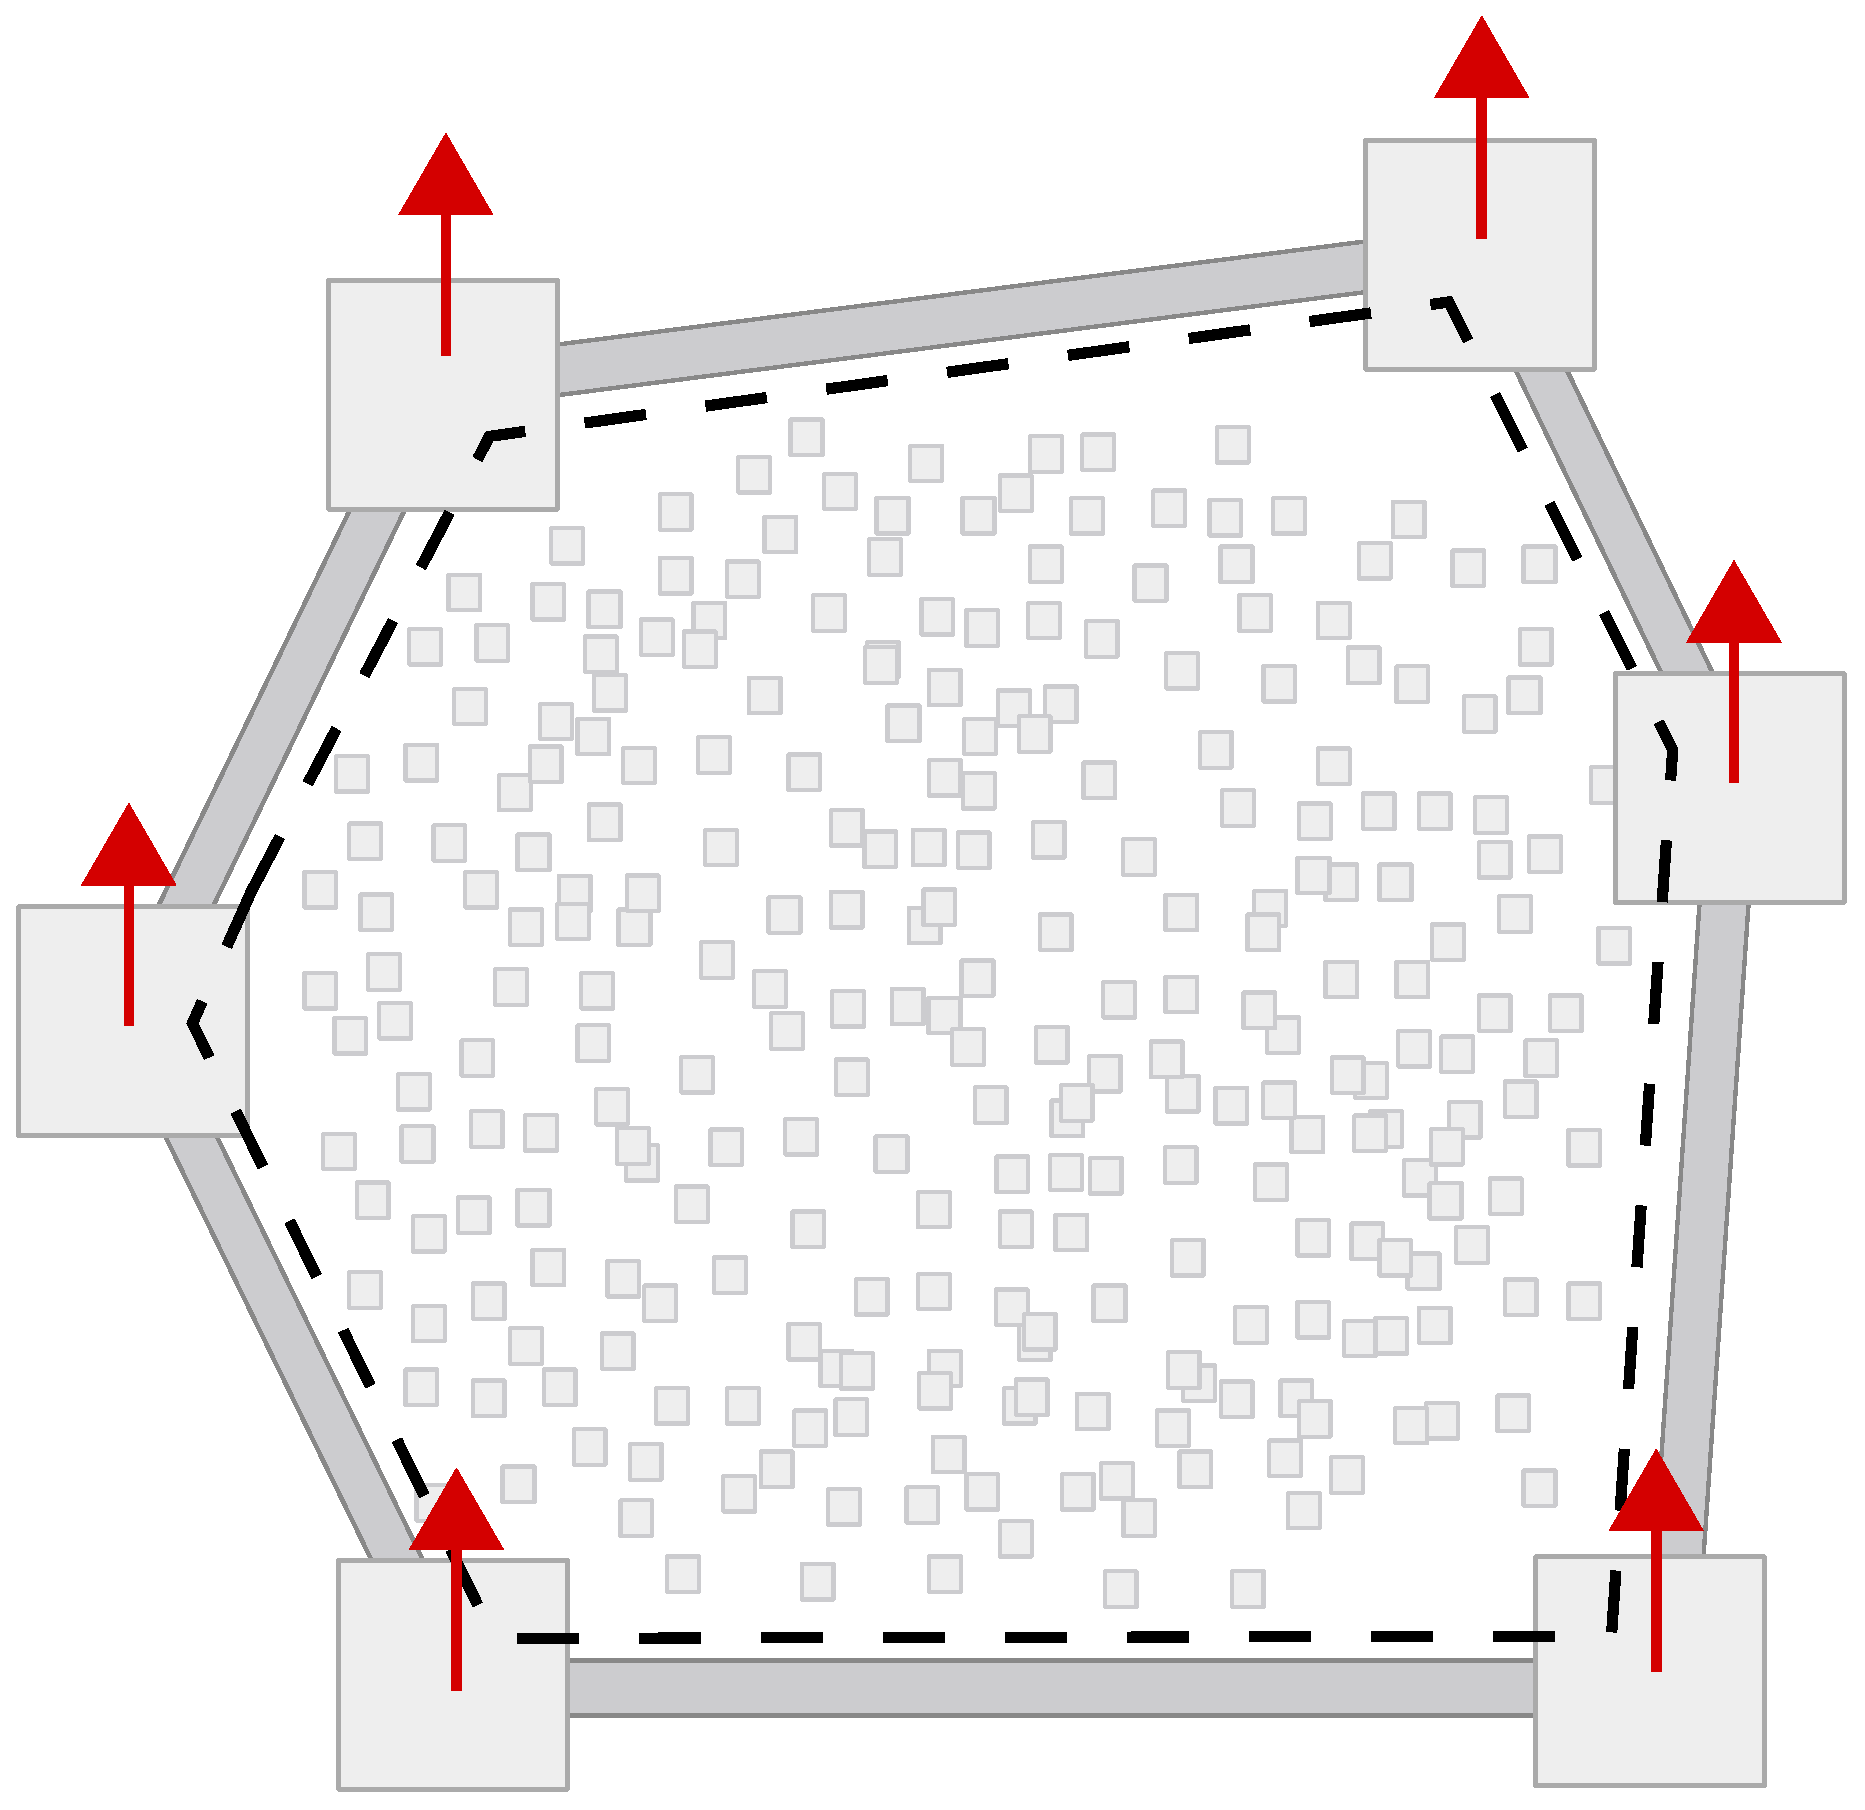
\includegraphics[width=2.5in]{figs/cityevolution_castle}
  \caption{Castle initial shape from old city bounding and castle oriented squared towers .}
  \label{fig:cityevolution_castle}
\end{figure}


 

 
\subsection{City Evolutions}
\label{sec:cityevolutions}
 
 This element contains a list of city evolution patterns. Each pattern defines the range time and the main direction of the city growth (in houses).
 The patterns can intersect in time with other patterns. 
 The evolution patterns are joined in groups wrapped by tag \texttt{<Group></Group>}, where each group is defined as follows:
 
 \begin{tabularx}{0.48\textwidth}{ |l|X| }
\hline 
\textbf{Parameter} & \textbf{Description} \\[0.15cm]
 \hline
  \texttt{ID} & Group identifier. It is used to be related later by \texttt{CityExpansion} (see Section \ref{sec:cityexpansion}.\\
  \hline
  \texttt{Evolutions} & List of evolutions, where each evolution is wrapped by \texttt{<Evolution></Evolution>} tag.\\
 \hline
\end{tabularx} 

 Each evolution pattern is defined as follows:
 
\begin{tabularx}{0.48\textwidth}{ |l|X| }
\hline 
\textbf{Parameter} & \textbf{Description} \\[0.15cm]
 \hline
 \texttt{TimeRange} & Time range in years. Format example:\\
 & \\
 & \quad\texttt{[850, 1100]} \\
 & \\
 \hline
 \texttt{Direction} & Expansion 2D vector. See \texttt{SegmentBase} for more information. Format example: \\
 & \\
 & \quad\texttt{[-0.3, -0.5]} \\
 & \\
 \hline
 \texttt{HousesPerYear} & Number of houses created by year. Optional parameter (1 by default). You can use values lower than 1 to specify a slow city growth. \\ 
 \hline
 \texttt{SegmentBase} & Definition of a segment from where the houses start its deployment. The houses deployment starts along the segment and follows the \texttt{Direction} vector (see Figure \ref{fig:cityevolution_patterns}.
 Because the houses expansion are calculated using a cosine distribution, the distribution will be more grazing for a shorter segments, and more sparsed for a longer segments (see Figure \ref{fig:cityevolution_patterns2}). 
 This value is optional. 
 If it is not defined, the deployment uses the castle walls as initial segments. The segment base is defined with 2 points. By example:\\
 & \\
 & \quad\texttt{<SegmentBase>}\\
 & \quad\quad\texttt{<P1>[23.1,24.2]</P1>}\\
 & \quad\quad\texttt{<P2>[34.4,25.6]</P2>}\\
 & \quad\texttt{</SegmentBase>}\\
 & \\
 \hline 
\end{tabularx} 

 
 
 
 
\begin{figure}[hp]
  \centering
  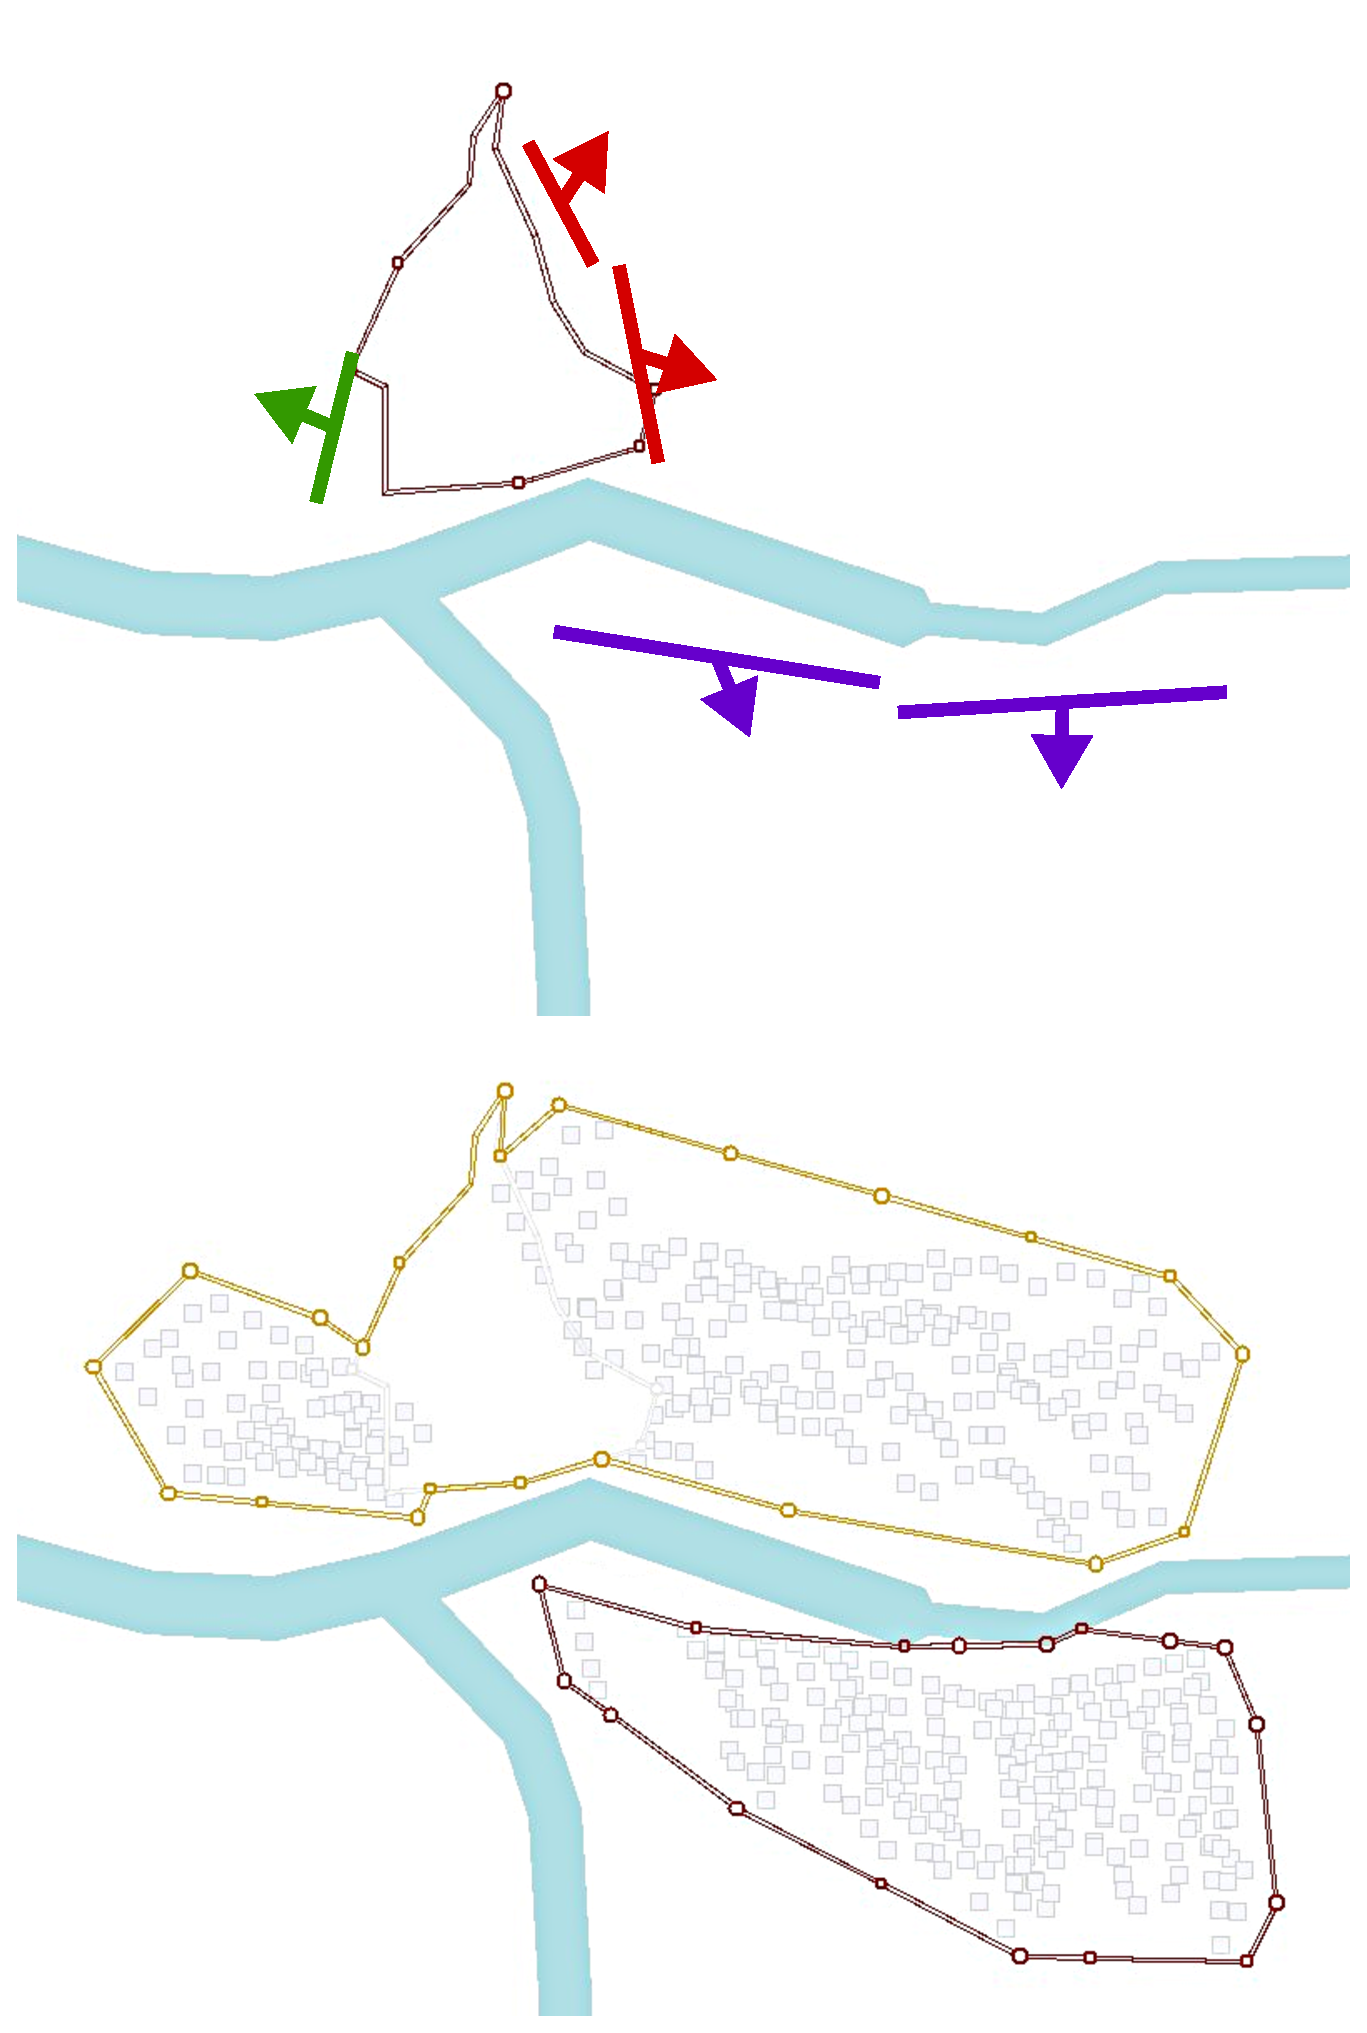
\includegraphics[width=3.25in]{figs/cityevolution_patterns}
  \caption{Example of city expansion using evolution patterns. There are three expansion groups, each one defined by a different arrow color.}
  \label{fig:cityevolution_patterns}
\end{figure}





 
\begin{figure}[hp]
  \centering
  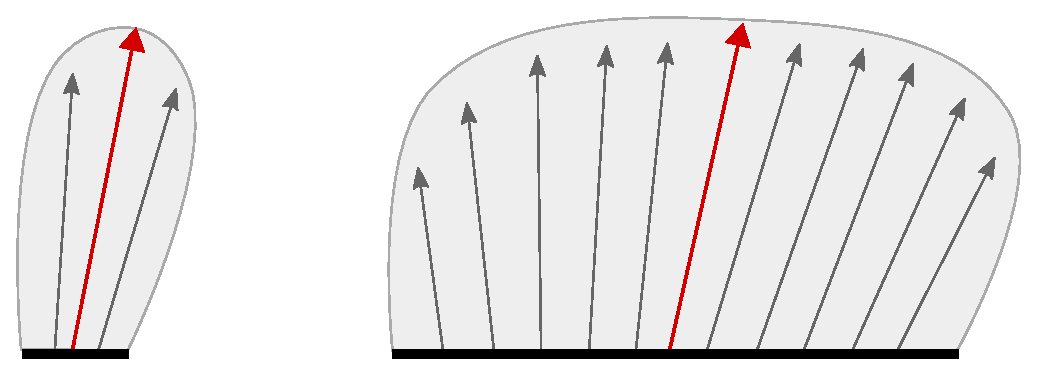
\includegraphics[width=3.25in]{figs/cityevolution_patterns2}
  \caption{Houses distribution differences between short and long base segments. }
  \label{fig:cityevolution_patterns2}
\end{figure}


 
\subsection{City Expansion}
\label{sec:cityexpansion}

The city expansion is executed when the castle is wrapped by a new curtain wall. 
This expansion can be generated by a defeat in a battle or manually using this section data.
This section is optional.

\begin{tabularx}{0.48\textwidth}{ |l|X| }
\hline 
\textbf{Parameter} & \textbf{Description} \\[0.15cm]
 \hline
   \texttt{WallDimensions} & Minimum and maximum wall lengths for all expansions. This parameter is usefull when the user wants to override the default settings value. Format example: \\
   & \\
   & \quad\texttt{[80.0, 150.0]} \\
   & \\
   & , where the values are respectively the minimum and maximum wall lengths.\\
 \hline
   \texttt{Expansion} & Defines the expansion year. Many expansions can be defined, each one related by the tag \texttt{<ID></ID>} to a \texttt{CastleEvolution} group. Format example:\\
 & \quad\texttt{<Expansion>}\\
 & \quad\quad\texttt{<Year>1384</Year>}\\
 & \quad\quad\texttt{<GroupID>1</GroupID>}\\
 & \quad\texttt{</Expansion>}\\
 & \\
 \hline
 \texttt{YearsBetween} & \\
 \texttt{Expansions} & Defines the number of years between city expansions due to battles and manual expansions. 
 If a close battle in time created a new castle, manual expansion is discarded, and viceversa. It is optional\\
\hline
\end{tabularx} 
 
 
 
\subsection{Battle events}
\label{sec:battleevents}

A set of battle simulation can be defined to be executed in a selected year.
Each battle event is wrapped by \texttt{<Battle></Battle>} tag. 
Each battle has the next parameters:

\begin{tabularx}{0.48\textwidth}{ |l|X| }
\hline 
\textbf{Parameter} & \textbf{Description} \\[0.15cm]
 \hline
 \texttt{Year} & Year of the battle \\
 \hline
 \texttt{Simulations} & Number of simulations. If it is 1, the battle is displayed. Otherwise, it runs in background and shows at the end a list of statistical results. \\
 \hline
 \texttt{RepeatUntil} & \\
 \texttt{DefendersWin} & If is true, the simulation loops until defender army wins or until the castle cannot be upgraded more.\\
 \hline
 \texttt{Defenders} & Defender army definition. See below.\\
 \hline
 \texttt{Attackers} & Attacker army definition. See below.\\
 \hline
\end{tabularx} 

The defenders army, wrapped with \texttt{<Defenders></Defenders>} tag, is defined by the number of ``\texttt{Archers}'' and ``\texttt{Cannons}'' to deploy.
The units are deployed automatically.
\newline

\begin{tabularx}{0.48\textwidth}{ |l|X| }
\hline 
\textbf{Parameter} & \textbf{Description} \\[0.15cm]
 \hline
 \texttt{Archers} & Number of archers to deploy. \\
 \hline
 \texttt{Cannons} & Number of cannons to deploy. They are deployed on towers before the archers deployment. Then the archers are deployed on the walls and on the empty spaces between cannons on the towers. There must be enough space in towers to deploy the towers (tower width and cell size). \\
 \hline
\end{tabularx} 
 



The attackers army are defined as a list of flanks \texttt{<Flank></Flank>}.
Each flank is a set of battalions that approach to the castle and attack it.
The parameters of a flank are: 

\begin{tabularx}{0.48\textwidth}{ |l|X| }
\hline 
\textbf{Parameter} & \textbf{Description} \\[0.15cm]
 \hline
 \texttt{Direction} & Flank attack direction. If origin is not specified, the flank advances in a directional way. Optional. Format example: \\
 & \\
 & \quad\texttt{[0.7, 0.7]} \\
 & \\
 \hline
 \texttt{Origin} & Flank origin position. Optional. Format example: \\
 & \\
 & \quad\texttt{[100.0, 100.0]} \\
 & \\ 
 \hline
 \texttt{StandDistance} & Distance from the castle bounding where the attackers start the battle. \\
 \hline
\end{tabularx} 

If none origin is specified, the vector is used to intersect a directional ray to the castle bounding circle with increased radius by the stand distance (see case $A$ in Figure \ref{fig:battle_events}). 
Then, the intersection point is the battalion deployment point.
If origin is specified but not the stand distance, the troops are deployed on the origin position.
If origin and stand distance are specified, the troops are deployed  on the intersection point between the castle bounding circle with increased radius by the stand distance, and the ray created with origin and direction  (see case $B$ in Figure \ref{fig:battle_events}).
Finally, if neither direction and origin are specified, a random vector is used in the same way if only direction was specified.

 
\begin{figure}[h]
  \centering
  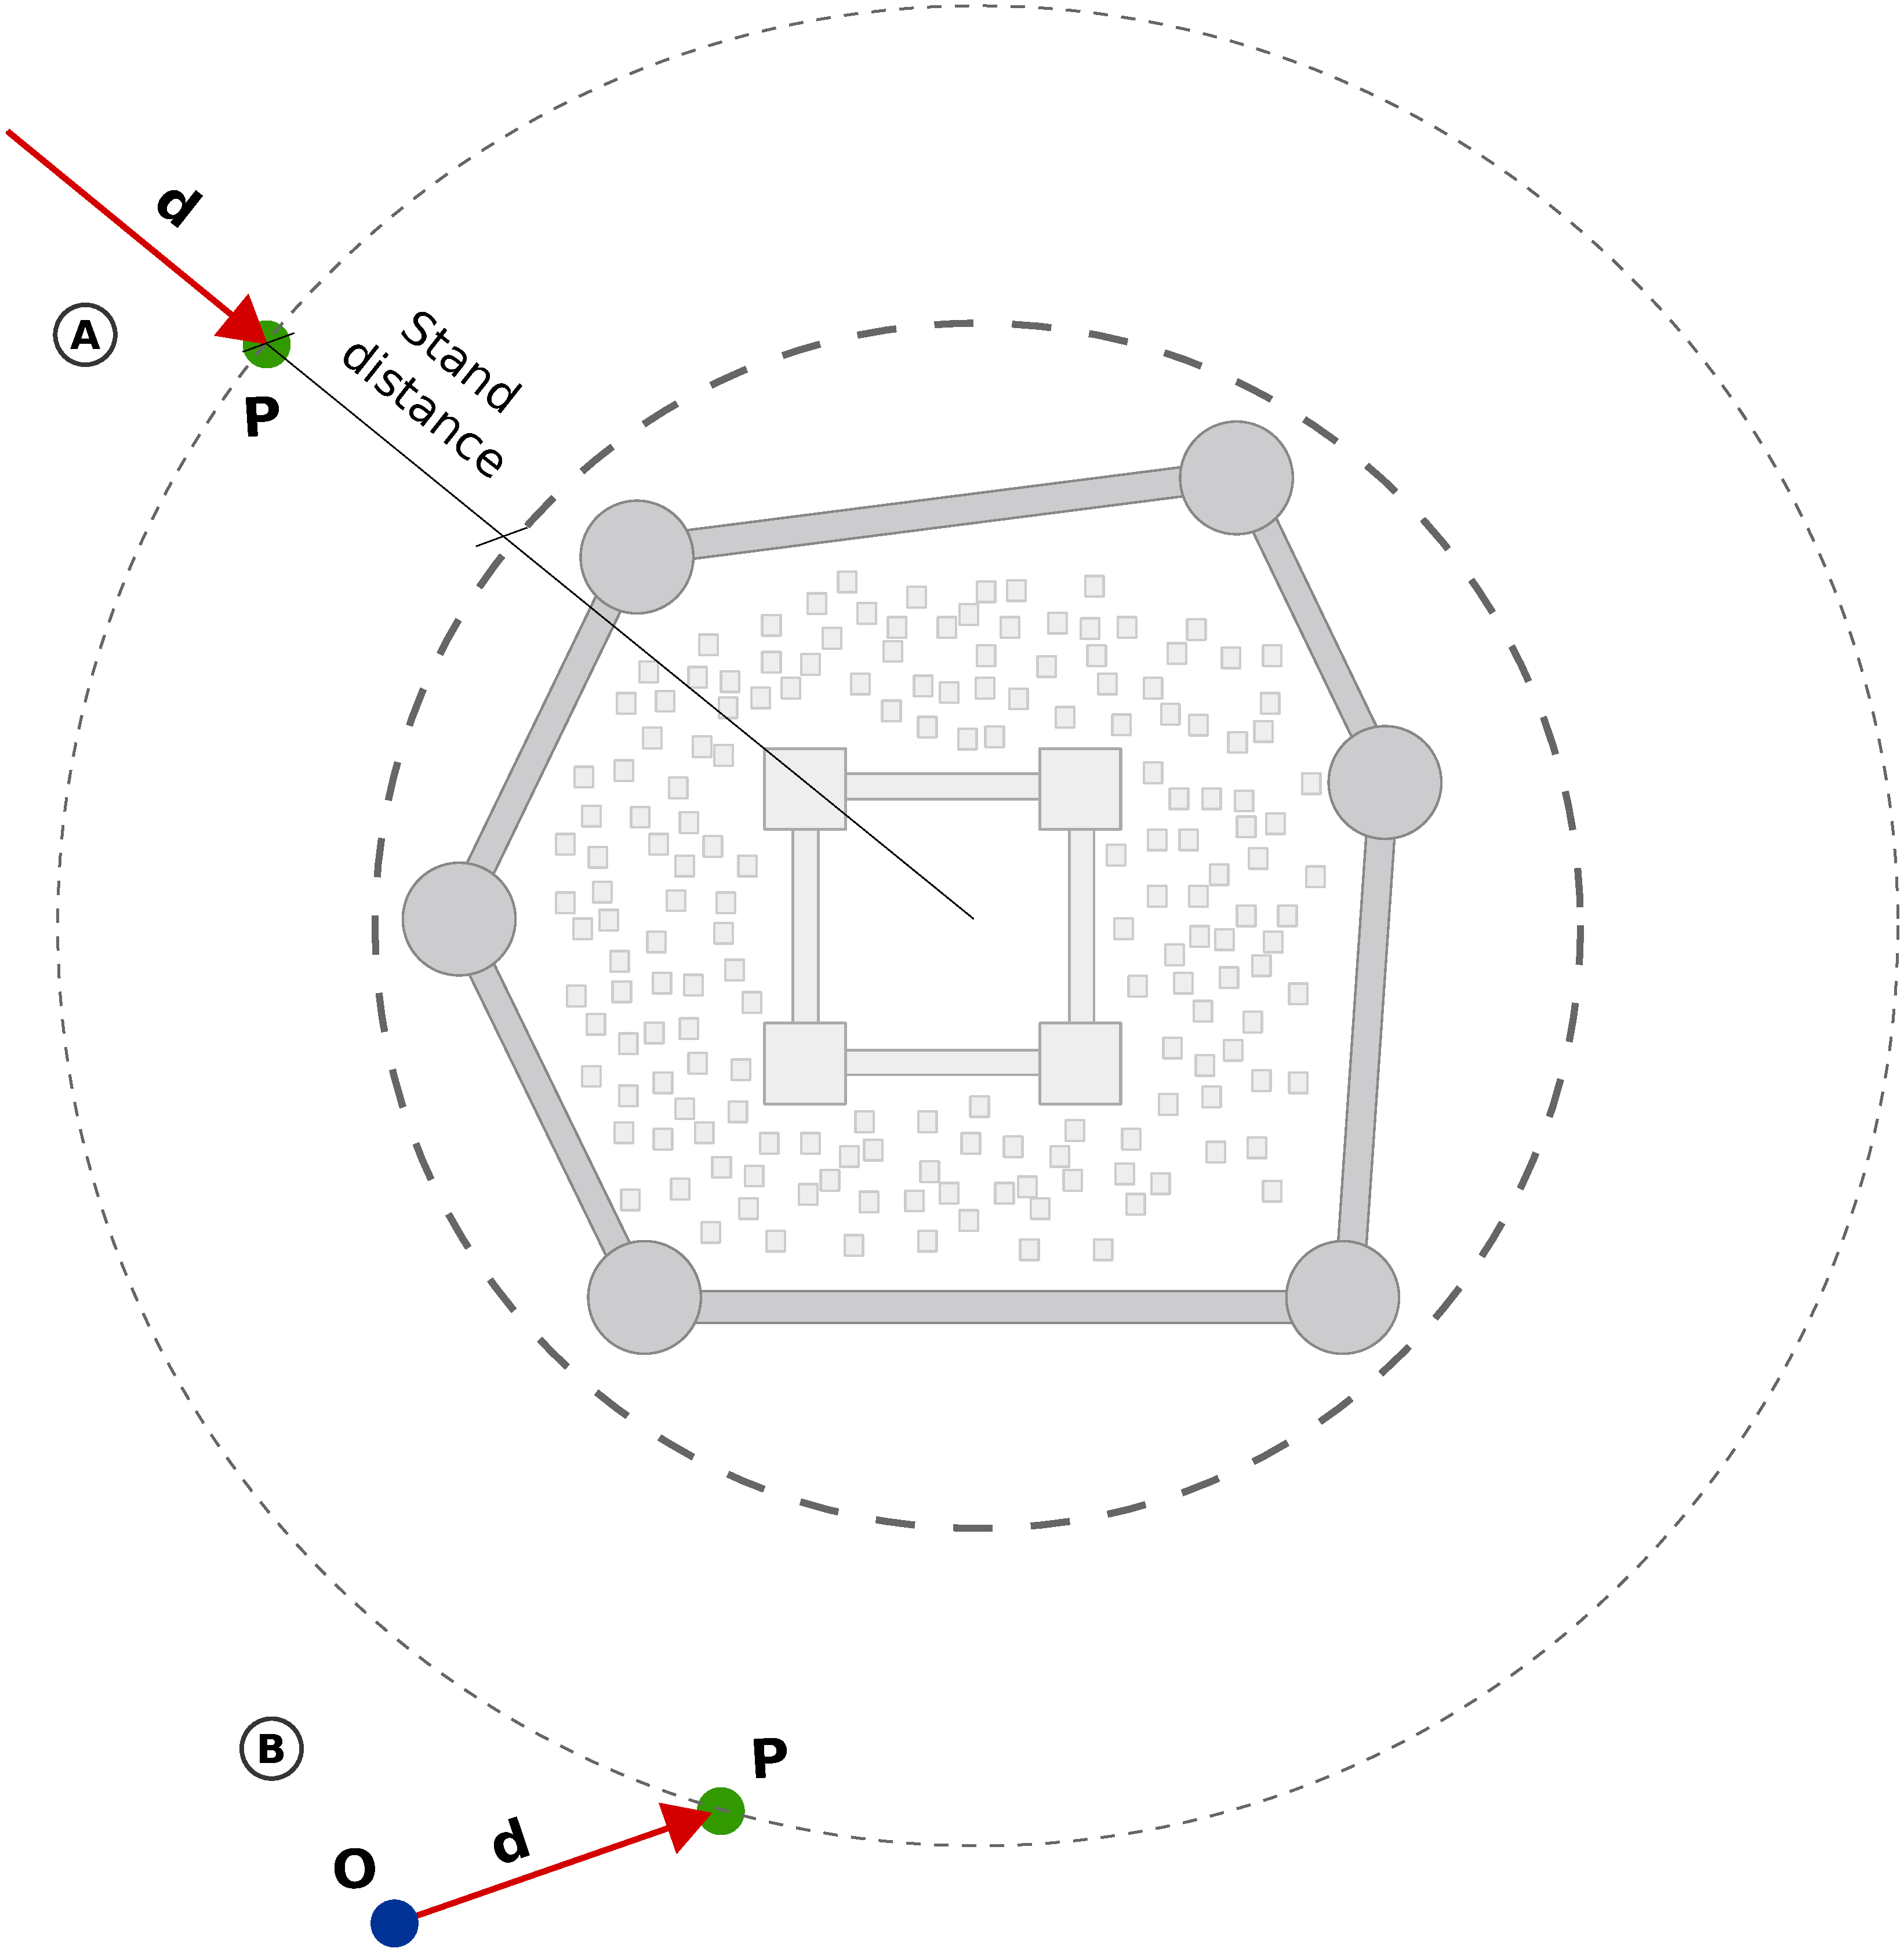
\includegraphics[width=3.25in]{figs/battle_events}
  \caption{Flank placement methods. Placement $P$ by only direction vector $d$ (case $A$), or placement by origin position $O$ and direction vector $d$ (case $B$). }
  \label{fig:battle_events}
\end{figure}
 
 
 
In addition, each flank defines a list of battalions, enclosed by \texttt{<Battalions></Battalions>} tag.
Each battalion, enclosed by \texttt{<Battalion></Battalion>} tag, has the next parameters:


\begin{tabularx}{0.48\textwidth}{ |l|X| }
\hline 
\textbf{Parameter} & \textbf{Description} \\[0.15cm]
 \hline
 \texttt{Type} & Type of battalion. The avaliable battalions are ``\texttt{Infantry}``, ''\texttt{Archers}``, ''\texttt{Cannons}`` and ''\texttt{SiegeTowers}``. \\
 \hline
 \texttt{Number} & Number of battalion units. \\
 \hline
 \texttt{BattalionSize} & Maximum battalion size for each battlefield cell. Optional. If it is not specified, the selected battlefield cells will be full populated. The battalion size is taken into account to populate the cell (see global settings). \\
 \hline
 \texttt{GroupSize} & Grouping size. Allows to deploy groups of battalions with a distance between them defined by GroupsDistance (see Figure \ref{fig:battalion_groups}). This parameter is usefull for deploy sparsed cannons batteries. Optional. 1 by default \\
 \hline
 \texttt{GroupDistance} & Distance between groups. Optional \\
 \hline
\end{tabularx} 


 
\begin{figure}[h]
  \centering
  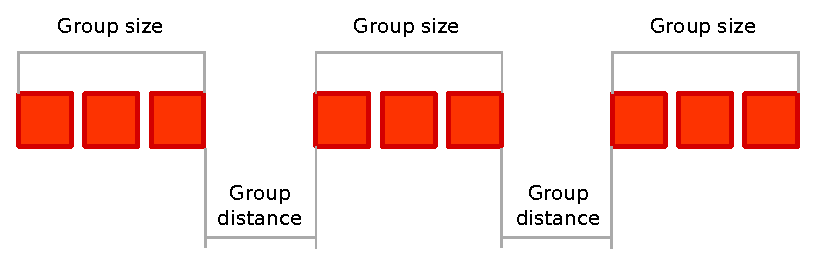
\includegraphics[width=3.25in]{figs/battalion_groups}
  \caption{Battalion grouping. }
  \label{fig:battalion_groups}
\end{figure}
 
 

Once the deployment starting position is calculated, the battalions deployment around it follow the next rules (see Figure \ref{fig:battalion_deployment}):

\begin{itemize}
 \item The first defined battalion is deployed at stand position. The deployment starts at calculated position and sparses the units along the flank direction perpendicular vector, in both sides.
 \item The next battalion is deployed just behind the first battalion deployment position. The same for the other battalions. So, the order is important.
 \item If the deployment of a battalion finds an obstacle (trenches, houses, any castle part or other battalions, jump to the behind row and continues the deployment.
 \item Battalions of the same kind can be repeated.
 \item The cannons deployment could be automatically changed if the final stand distance is too close or too far from the castle. See the cannon shoot parameters at global settings.
 \item The siege towers need a clear and straight path to any castle wall. So, the siege towers could be deployed far from their initial deployment position, searching the best attack position and direction.
\end{itemize}

\begin{figure}[h]
  \centering
  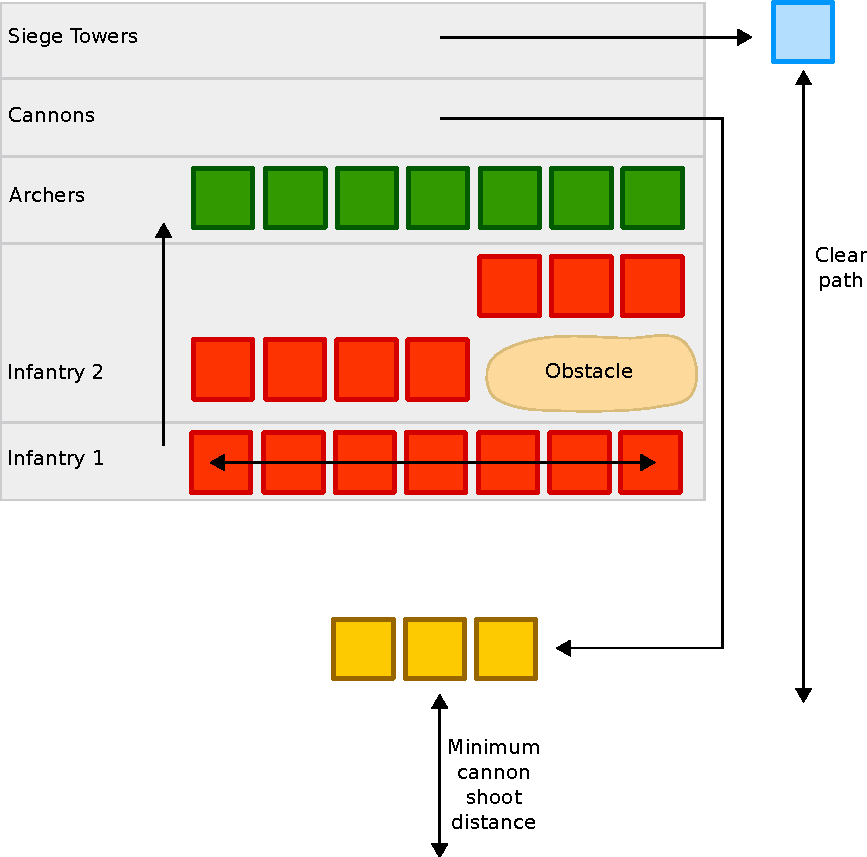
\includegraphics[width=3.25in]{figs/battallion_deployment}
  \caption{Battalion deployment on the battlefield. }
  \label{fig:battalion_deployment}
\end{figure}




\subsection{Expansion checkings}
\label{sec:expansioncheckings}

This element is a list of years where the expanion history is printed out. It is optional.

\begin{tabularx}{0.48\textwidth}{ |l|X| }
\hline 
\textbf{Parameter} & \textbf{Description} \\[0.15cm]
 \hline
 \texttt{Year} & Checking year \\
 \hline
\end{tabularx} 



\subsection{Star Fortress}
\label{sec:starfortress}

The star fortress is an optional final expansion castle shape.
The result is not applicable to any battle, so this shape is calculated at the end of the simulation if it is specified.
The next table shows the parameters to construct the star fortress. 


\begin{tabularx}{0.48\textwidth}{ |l|X| }
\hline 
\textbf{Parameter} & \textbf{Description} \\[0.15cm]
 \hline
  \texttt{Activate} & \texttt{True} to activate the star fortress shape, or \texttt{False} otherwise (or just not define \texttt{StarFortress} section. \\
  \hline
%   \texttt{BastionRadius} & The bastions are constructed by the circle method (see description of this method on the main documentation). If there are non-bastion towers at the moment of the star fortress construction, they are converted to bastions using this circle radius to calculate the new geometry. Default value: 40.0\\
%  \hline
%  \texttt{Ravelin} & The ravelins construcions have two parameters: \\
%  & \quad\texttt{Radius}: Circle radius to construct ravelins (like bastions). Default value: 40.0 \\
%  & \quad\texttt{MinWidth}: Minimum ravelin width. Used to avoid too thin ravelins. Default value: 15.0\\
%  \hline
%  \texttt{HalfMoon} & The halfmoons are optional. Their parameters are: \\
%  & \quad\texttt{Activate}: \texttt{True} to activate them. Default value: \texttt{True}\\
%  & \quad\texttt{CircleOffset}: Distance between halfmoon center and halfmoon circle radius. Default value: 5.0\\
%  & \quad\texttt{Length}: Distance from the halfmoon circle center to the halfmoon jag. Default value: 30.0\\
%  \hline
%  \texttt{CovertWay} & The covert way is mandatory, so it wraps the castle, ravelins and halfmoons. Its parameters are: \\
%  & \quad\texttt{Thickness}: Thickness of the covert way. Default value: 10.0 \\
%  & \quad\texttt{Offset}: Distance from the halfmoons/ravelins to the covertway. Default value: 5.0 \\
%  & \quad\texttt{HasPlacesOfArms}: \texttt{True} if places of arms have to be constructed on each non-convex angle of the covertway external shape. Default value: \texttt{True}\\
%  & \quad\texttt{PlacesOfArmsLength}: Length of the squared places of arms. Default value: 10.0\\
%  \hline
%  \texttt{GlacisThickness} & Thickness of the glacis, the outer wrapper to the covertway, and the most external star fortress defense. Default value: 10.0 \\
%  \hline
\end{tabularx} 

See Section \ref{sec:settingscastlestarfortress} to know how to change the default parameters.



\section{Simulation XML: Battles}
\label{sec:battle}

The user can test and check specific battles out of the city evolution context. To do it the \texttt{Type} parameter must be defined as \texttt{Battle}.
The XML structure is different from the city evolution mode, so both parameters cannot be mixed.
This simulation mode is just for checking and debuging purposes, and it does not calculate weakest points in the castle structure.
The parameters for this play mode are shown on the next table. All of them are mandatory except those that are indicated as optional.

\begin{tabularx}{0.48\textwidth}{ |l|X| }
\hline 
\textbf{Parameter} & \textbf{Description} \\[0.15cm]
 \hline
 \texttt{Period} & Century of the simulation. Used to select the kind of towers. See Section \ref{sec:settingscastletower}.\\
 \hline
 \texttt{Battlefield} & Battlefield definition. See Section \ref{sec:battlebattlefield}. \\
 \hline
 \texttt{Castle} & Castle definition. See section \ref{sec:battlecastle}. \\
 \hline
 \texttt{AttackersPopulate} & Attackers army definition and deployment. See Section \ref{sec:battleattackers}. \\
 \hline
 \texttt{DefendersPopulate} & Defenders army definition. See Section \ref{sec:battledefenders}. \\
 \hline
 \texttt{HasHeightViews} & \texttt{True} if the wall height views have to be shown. \\
 \hline
\end{tabularx} 



\subsection{Battlefield}
\label{sec:battlebattlefield}

This element is defined as seen in Section \ref{sec:battlefield}.
In addition, it includes in this mode the trenches manual definition.
If it is not defined, the trenches are created automatically (see global settings).

\begin{tabularx}{0.48\textwidth}{ |l|X| }
\hline 
\textbf{Parameter} & \textbf{Description} \\[0.15cm]
 \hline
 \texttt{Bounding} & Battlefield size \\
 \hline
 \texttt{CellSize} & Battlefield cell size \\
 \hline
 \texttt{Trenches} & List of lists of cell coordinates by their indices. Each list is wrapped by a \texttt{<Set></Set>} tag. Format example: \\
 & \\
 & \texttt{<Set>[[20,7], [21,7], [22, 7], [23, 7]</Set>} \\
 & \texttt{<Set>[[8, 8], [8, 9]]</Set>} \\
 & \\
 \hline
\end{tabularx} 




\subsection{Castle}
\label{sec:battlecastle}

This element is also defined as seen in Section \ref{sec:castle}.
In addition, it includes in this mode the moat activation. If it is not specified the moat is deactivated by default. It is optional.

\begin{tabularx}{0.48\textwidth}{ |l|X| }
\hline 
\textbf{Parameter} & \textbf{Description} \\[0.15cm]
 \hline
 \texttt{Orientation} & Castle orientation 2D vector. \\
 \hline
 \texttt{OldCity} & List of \texttt{<House></House>} with the inner castle houses. \\
 \hline
 \texttt{Moat} & Set the value of \texttt{<HasWater></HasWater>} to \texttt{True} or \texttt{False} to activate the water covered moat or not. \\
 \hline
\end{tabularx} 
 
Check the default values in global settings to define the moat parameters such are depth or width.



\subsection{Attackers army}
\label{sec:battleattackers}

The attacker army deployment differs from the city evolution mode. 
The parameters are defined on the next table: 

\begin{tabularx}{0.48\textwidth}{ |l|X| }
\hline 
\textbf{Parameter} & \textbf{Description} \\[0.15cm]
 \hline
 \texttt{ArmySize} & List with all kinds of attacker army battalions and their sizes. Available battalions are ''\texttt{Infantry}``, ''\texttt{Archers}``, ''\texttt{Cannons}`` and ''\texttt{SiegeTowers}``. Format example:  \\
 & \\
 & \quad\texttt{<Battalion>} \\
 & \quad\quad \texttt{[}''\texttt{Infantry}``\texttt{, 7000]} \\
 & \quad\texttt{</Battalion>} \\
 & \\
 \hline
 \texttt{Battalion} & See below \\
 \hline
\end{tabularx} 

Each battalion is deployed by a list of elements wrapped by \texttt{<Battalion></Battalion>}. The parameters are shown on the next table
The placement is manual, defined by regions. 
The user can specify cell ranges where to deploy battalions of the same kind.
An infantry battalion should be specified as minimum, so the simulation ends when the defenders army defeats or when the attacker army infantry defeats, that is any infantry unit can climb any castle wall.

\begin{tabularx}{0.48\textwidth}{ |l|X| }
\hline 
\textbf{Parameter} & \textbf{Description} \\[0.15cm]
 \hline
 \texttt{Type} & Type of battalion. The available types are ''\texttt{Infantry}``, ''\texttt{Archers}``, ''\texttt{Cannons}`` and ''\texttt{SiegeTowers}``. \\
 \hline
 \texttt{DeploymentByRange} & Range of cells where to deploy the battalions. The cells are specified by their indices. Format example: \\
 & \\
 & \quad\texttt{<First>} \\
 & \quad\quad\texttt{[3, 3]} \\
 & \quad\texttt{</First>} \\
 & \quad\texttt{<Last>} \\
 & \quad\quad\texttt{[3, 46]} \\
 & \quad\texttt{</Last>} \\
 & \\
 & This deployment overrides the standard deployment method seen in Figure \ref{fig:battalion_deployment}.\\
 \hline
 \texttt{BattalionSize} & Battalion size for each battlefield cell. Optional. -1 by default (populate the whole cell) \\
 \hline
 \texttt{SiegeTowerNumber} & Number of siege towers to deploy. The siege towers are deployed automatically, choosing front positions to the weakest walls. This property is only avaiable for siege towers deployments. If it is used, \texttt{DeploymentByRange} and \texttt{BattalionSize} are not considered. A siege tower needs one infantry battalion to use it as a turtle battalion, that will cover the moat. \\
 \hline
\end{tabularx} 



\subsection{Defenders army}
\label{sec:battledefenders}

The defenders are deployed automatically on the castle walls and towers. 
There are only two kind of battalions to deploy on a castle: ''\texttt{Archers}`` and ''\texttt{Cannons}''

\begin{tabularx}{0.48\textwidth}{ |l|X| }
\hline 
\textbf{Parameter} & \textbf{Description} \\[0.15cm]
 \hline
 \texttt{Archers} & Number of archers to deploy. \\
 \hline
 \texttt{Cannons} & Number of cannons to deploy. They are deployed on towers before the archers deployment. Then the archers are deployed on the walls and on the empty spaces between cannons on the towers. There must be enough space in towers to deploy the towers (tower width and cell size). \\
 \hline
\end{tabularx} 
 






\section{Settings XML}

If none \texttt{settingsxml} parameter is specified in \texttt{Run} class constructor, the default XML settings file is used.
It is located at \texttt{Battles/Utils/settings.xml}.
It is recommended to copy and edit it if some changes are needed. 

The structure is wrapped on \texttt{<Battles></Battles>} tag.
The parameters and elements are shown on the next table:

\begin{tabularx}{0.48\textwidth}{ |l|X| }
\hline 
\textbf{Parameter} & \textbf{Description} \\[0.15cm]
 \hline
 \texttt{Castle} & Castle and constructions defaults. See Section \ref{sec:settingscastle}. \\
 \hline
 \texttt{Battlefield} & Battlefield size and trenches. See Section \ref{sec:settingsbattlefield} \\
 \hline
 \texttt{Army} & Armies defaults, for defenders and attackers. See Section \ref{sec:settingsarmy} \\
 \hline
 \texttt{City} & City evolution defaults. See Section \ref{sec:settingscity} \\
 \hline
 \texttt{Game} & Some game miscellaneous parameters. See Section \ref{sec:settingsgame} \\
 \hline
\end{tabularx} 



\subsection{Castle}
\label{sec:settingscastle}

The castle parameters define the default values for the castle construction elements, such are walls, towers, moat or the star fortress.

\begin{tabularx}{0.48\textwidth}{ |l|X| }
\hline 
\textbf{Parameter} & \textbf{Description} \\[0.15cm]
 \hline
  \texttt{Orientation} & Castle front direction. It is used as reference to construct well oriented squared towers. \\
  & The value is a 2D vector. Format example:  \\ 
  & \\
  & \quad\texttt{[0.0, -1.0]}\\
  & \\
 \hline
 
 
 \texttt{CurtainWall} & \\
 \texttt{OldCityMargin} & Margin around the inner city to construct the initial wrapping curtain wall. \\
 \hline
 \texttt{DefendingLine} & Castle defensive lines settings. It has 3 parameters: \\
 & \\
 & \quad\texttt{Width}: Wall/tower walkway free space to deploy archers. \\
 & \quad\texttt{CellSize}: Available free space to deploy an unit on the wall. \\
 & \quad\texttt{Height}: Baseline height from the wall/tower walkway. \\
 & \\
 \hline
\end{tabularx} 


 \begin{tabularx}{0.48\textwidth}{ |l|X| }
\hline 
\textbf{Parameter} & \textbf{Description} \\[0.15cm]
 \hline
\texttt{ShowLabels} & Set to \texttt{True} to show each castle construction element label. \\
 \hline
 \texttt{Wall} & See Section \ref{sec:settingscastlewall}. \\
 \hline
 \texttt{Tower} & See Section \ref{sec:settingscastletower}. \\
 \hline
 \texttt{Bastion} & See Section \ref{sec:settingscastlebastion}. \\
 \hline 
 \texttt{Moat} & See Section \ref{sec:settingscastlemoat}. \\
 \hline
 \texttt{StarFortress} & See Section \ref{sec:settingscastlestarfortress}. \\
 \hline
\end{tabularx} 



\subsubsection{Walls}
\label{sec:settingscastlewall}

The walls parameters are shown on the next table.

\begin{tabularx}{0.48\textwidth}{ |l|X| }
\hline 
\textbf{Parameter} & \textbf{Description} \\[0.15cm]
 \hline
 \texttt{InnerHeight} & Wall height. \\
 \hline
 \texttt{Thickness} & Wall thickness. \\
 \hline
 \texttt{MerlonHeight} & Merlons height. Used to calculate the walkway heigth. Barely used. At least, it should not be negative or too high. \\
 \hline
 \texttt{WalkwayWidth} & Walkway width. It should be enough big to allow the archer units deployment. Barely used. \\
 \hline
 \texttt{DefenseIncrease} & Increase defenders defense factor due the wall protection. \\
 \hline
 \texttt{BattalionGrid} & \\
 \texttt{CellSize} & Available free space for each deployed unit on the wall. Currently, only archers are allowed to be deployed on walls. \\
 \hline
 \texttt{DefenseAngle} & Angle ranges that permit the wall defense. It has two parameters: \\
 & \\
 & \quad\texttt{H}: 2D plain view angle (degrees) around the main attack vector (wall normal vector). \\
 & \quad\texttt{V}: Vertical angles (in height), from bottom to main attack vector, and from this vector to top. \\
 & \\
 \hline
 \texttt{Tile} & Default parameters for the wall tiles. They have four parameters: \\
 & \\
 & \texttt{Width}: Tile width. \\
 & \texttt{Height}: Tile height. \\
 & \texttt{Resistance}: Tile resistance. The value, applied to each tile, is decreased as it receives cannon ball impacts. \\
 & \texttt{RubbleConversionFactor}: When a cannon ball impacto to a tile, a part of the tile material is converted to rubble that falls to the floor. The parameter value is the percentages of rubble that fall at tile left, front and right sides (see Figure \ref{fig:wallbreak}). Format example: \\
 & \\
 & \quad\texttt{[0.25, 0.5, 0.25]} \\
 & \\
 \hline
\end{tabularx} 

\begin{figure}[ht]
  \centering
  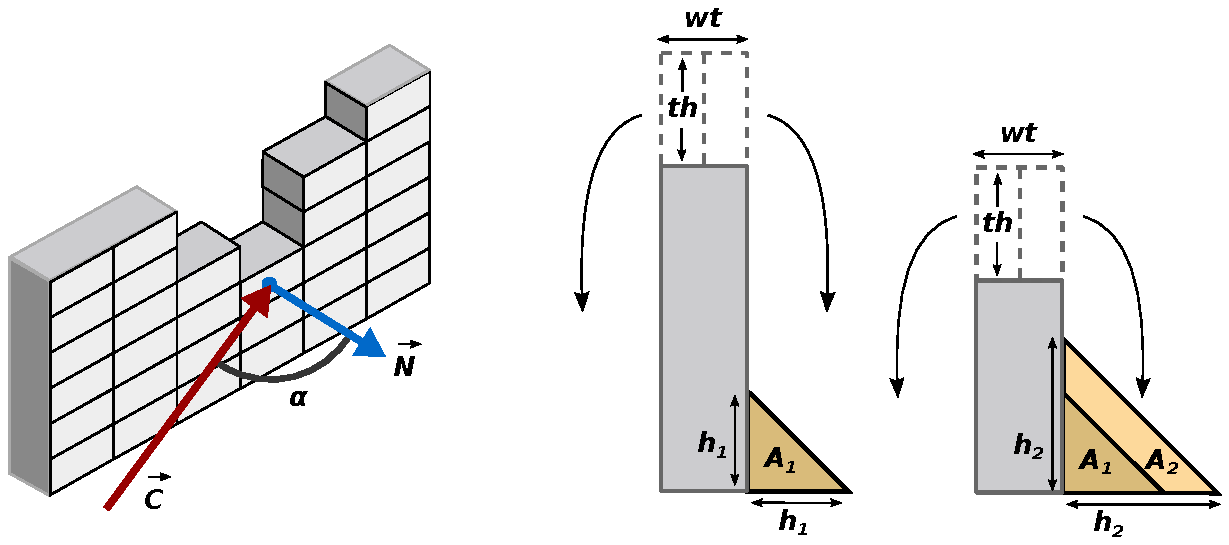
\includegraphics[width=3.25in]{figs/wallbreak}
  \caption{Wall breaking by cannon shoots on wall tiles (left). When a tile is broken, its material falls down creating a slope (center and right), where $wt$ is the wall thickness and $th$ is the tile height.}
  \label{fig:wallbreak}
\end{figure}



\subsubsection{Towers}
\label{sec:settingscastletower}

There are three kind of towers: squared, rounded and bastions.
The tower type selection is done automatically considering the century of creation.
Althought the bastion is a kind of tower due it is also a construction element that join walls, it is explained at the next section due it has a different set of parameters.
In addition, some of the next values are used too for bastions.

The towers parameters are shown on the next table:

\begin{tabularx}{0.48\textwidth}{ |l|X| }
\hline 
\textbf{Parameter} & \textbf{Description} \\[0.15cm]
 \hline
 \texttt{TimeRange} & Ranges of centuries to choose the type of tower to construct. The ranges should overlap, so the system uses a fuzzy algorithm between them. There are three time ranges: \texttt{Squared}, \texttt{Rounded} and \texttt{Bastion}. \\
 \hline
 \texttt{InnerHeight} & Tower height. \\
 \hline
 \texttt{Thickness} & Tower thickness. This value should be enough big to allow the cannons deployment. \\
 \hline
 \texttt{SquareSide} & Length of squared tower side. \\
 \hline
 \texttt{CircleRadius} & Radius of rounded tower. \\
 \hline
 \texttt{DefenseIncrease} & Increase defenders defense factor due the tower protection. Used also for bastions.\\
 \hline
 \texttt{BattalionGrid} & \\
 \texttt{CellSize} &  Available free space for each deployed unit on the tower. Due the towers allow the cannons and archers deployment, it has two values: \\
 & \\
 & \quad\texttt{Large}: Space to deploy a cannon. \\
 & \quad\texttt{Small}: Space to deploy an archer. \\
 & \\
 \hline
\end{tabularx}  
 
\begin{tabularx}{0.48\textwidth}{ |l|X| }
\hline 
\textbf{Parameter} & \textbf{Description} \\[0.15cm]
 \hline
 \texttt{DefenseAngle} & Angle ranges that permit the tower defense. Used also for bastions. It has two parameters: \\
 & \\
 & \quad\texttt{H}: 2D plain view angle (degrees) around the main attack vector. The main vector for rounded towers is the radial vector. For the squared ones and bastions, the main vector depends on the side, that is each side normal vector. \\
 & \quad\texttt{V}: Vertical angles (in height), from bottom to main attack vector, and from this vector to top. \\
 & \\
 \hline
 \texttt{RequiredDistance} & \\
 \texttt{NeighborFactor} & Value multiplied by the required free distance around a tower to place another one. It is recommended to use values greater than 2. It is optional. The default value is 3.\\
 \hline
\end{tabularx} 





\subsubsection{Bastion}
\label{sec:settingscastlebastion}
 
The bastion settings are shown on the next table.
Bastions also use some tower settings (see last section).

\begin{tabularx}{0.48\textwidth}{ |l|X| }
\hline 
\textbf{Parameter} & \textbf{Description} \\[0.15cm]
 \hline
 \texttt{VirtualCircle} & \\
 \texttt{Radius} & Radius of the virtual rounded tower used to create the bastion. (see Figure \ref{fig:bastion}) \\
 \hline
 \texttt{Thickness} & Bastion wall thickness. The relation between the circle radius and thickness is important. The radius cannot be less than thickness. If both are close, the bastion will be almost closed. In this case, the system will clamp the radius to the thickness. \\
 \hline
 \texttt{Height} & Bastion height. \\
 \hline
 \texttt{BattalionGrid} & \\
 \texttt{CellSize} &  Available free space for each deployed unit on the bastion. Due the bastions allow the cannons and archers deployment, it has two values: \\
 & \\
 & \quad\texttt{Large}: Space to deploy a cannon. \\
 & \quad\texttt{Small}: Space to deploy an archer. \\
 & \\
 \hline
 \texttt{MinDistance} & Minimum distance between bastions. Used when the towers are transformed into bastions to construct the starfortress. If there is not enough free space to fit a new bastion, its size is decreased, or it is removed. \\
 \hline
\end{tabularx} 



\begin{figure}[h]
  \centering
  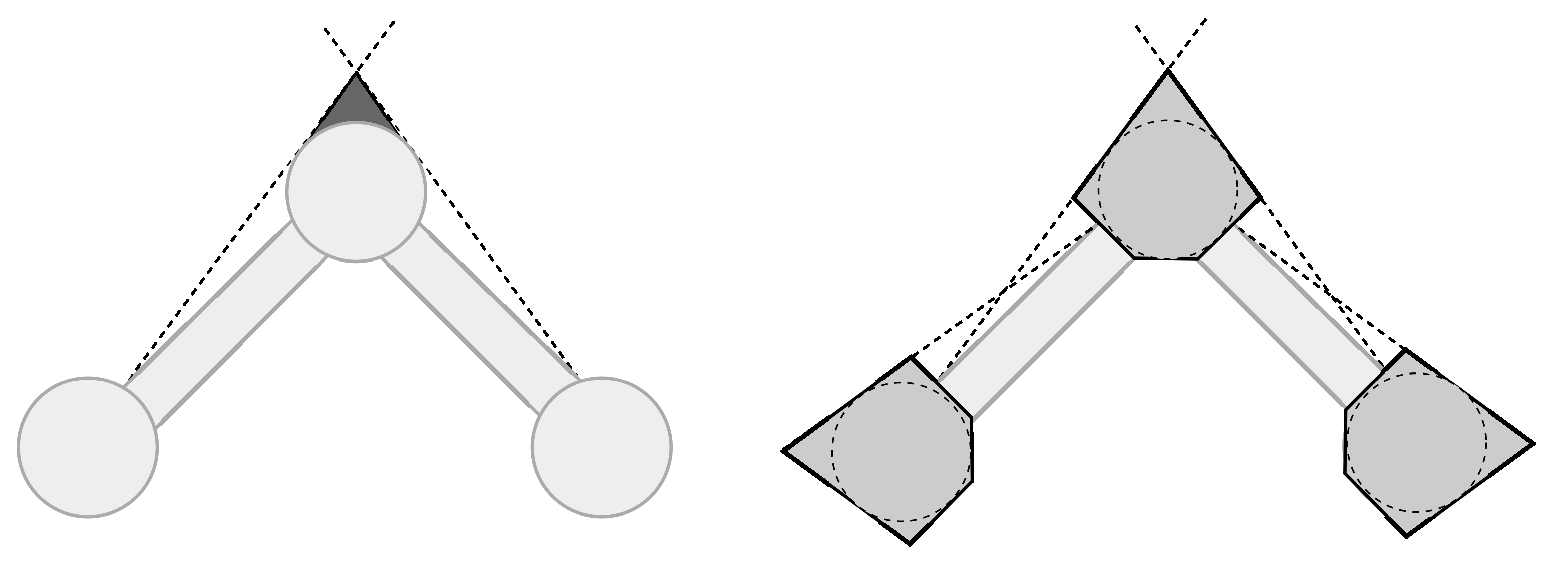
\includegraphics[width=3.25in]{figs/bastion}
  \caption{Bastion creation from rounded towers to cover blind spots. }
  \label{fig:bastion}
\end{figure}




\subsubsection{Moat}
\label{sec:settingscastlemoat}

The moat is automatically created around the curtain wall and towers.
The parameters that define it are: 

\begin{tabularx}{0.48\textwidth}{ |l|X| }
\hline 
\textbf{Parameter} & \textbf{Description} \\[0.15cm]
 \hline
 \texttt{Depth} & Moat depth. \\
 \hline
 \texttt{Width} & Moat width, or thickness in 2D plan view. \\
 \hline
 \texttt{HasWater} & Set to \texttt{True} if moat has water. \\
 \hline
 \texttt{PenaltyWater} & Penalty movement applied to battalions movement on the battlefield for watered moats. The value is a percentage that is multiplied by the itself battalion movement penalties. The value 1.0 means no penalty. \\
 \hline
 \texttt{PenaltyNoWater} & Like \texttt{PenaltyWater}, but applied on moats without water. \\
 \hline
\end{tabularx} 





\subsubsection{Star Fortress}
\label{sec:settingscastlestarfortress}

The next table shows the parameters to construct the star fortress. 
Some of star fortress elements are optional, such are half moons (\textit{lunettes}) and covert way.

\begin{tabularx}{0.48\textwidth}{ |l|X| }
\hline 
\textbf{Parameter} & \textbf{Description} \\[0.15cm]
 \hline
  \texttt{Ravelin} & The ravelins construcions have two parameters (see Figure \ref{fig:ravelin}): \\
  & \quad\texttt{Method}: Ravelin construction method. Values can be 1 or 2: \\
  & \quad\quad 1: Ravelin flanks constructed at \texttt{<BastionAngle>} from bastion flanks. \\
  & \quad\quad 2: Ravelin frontal length constructed with \texttt{<Radius>} distance. \\ 
  & \quad \textit{NOTE: Currently the method 1 is deprecated and should be checked before use it. Only for symmetric fortresses.} \\
  & \quad\texttt{BastionAngle}: Angle between bastion flanks and ravelin flanks. It shouldnt be less than 90 degrees. \\
  & \quad\texttt{Radius}: Circle radius to construct ravelins (like bastions).  \\
  & \quad\texttt{MinimumWidth}: Minimum ravelin width. Used to avoid too thin ravelins. \\
  \hline
  \texttt{HalfMoon} & The halfmoons (or \textit{lunettes}) are optional. Their parameters are (see Figure \ref{fig:halfmoon}): \\
  & \quad\texttt{Activate}: \texttt{True} to activate them.\\
  & \quad\texttt{CircleOffset}: Distance between halfmoon center and halfmoon circle radius.\\
  & \quad\texttt{Length}: Distance from the halfmoon circle center to the halfmoon jag. \\
  \hline
\end{tabularx}  
 
\begin{tabularx}{0.48\textwidth}{ |l|X| }
\hline 
\textbf{Parameter} & \textbf{Description} \\[0.15cm]
 \hline
  \texttt{CovertWay} & The covert way is mandatory, so it wraps the castle, ravelins and halfmoons. Its parameters are (see Figure \ref{fig:covertway}): \\
  & \quad\texttt{Thickness}: Thickness of the covert way. \\
  & \quad\texttt{Offset}: Distance from the halfmoons/ravelins to the covertway (see distance $d$ on Figure \ref{fig:covertway}). \\
  & \quad\texttt{PlaceOfArms}: \texttt{True} if places of arms have to be constructed on each non-convex angle of the covertway external shape.\\
  & \quad\texttt{PlaceOfArmsLength}: Length of the squared places of arms.\\
  & \quad\texttt{MinimumSegmentLength}: Minimum segment length of covert way polyline. Used to avoid wrong polylines with too small segments. \\
  & \quad\texttt{GlacisThickness}: Thickness of the glacis, the outer wrapper to the covertway, and the most external star fortress defense. \\
  \hline  
\end{tabularx} 


There are not any bad shape control method, so some parameter combinations could produce wrong shapes. 
The default values should work well for many castles.

\begin{figure}[ht]
  \centering
  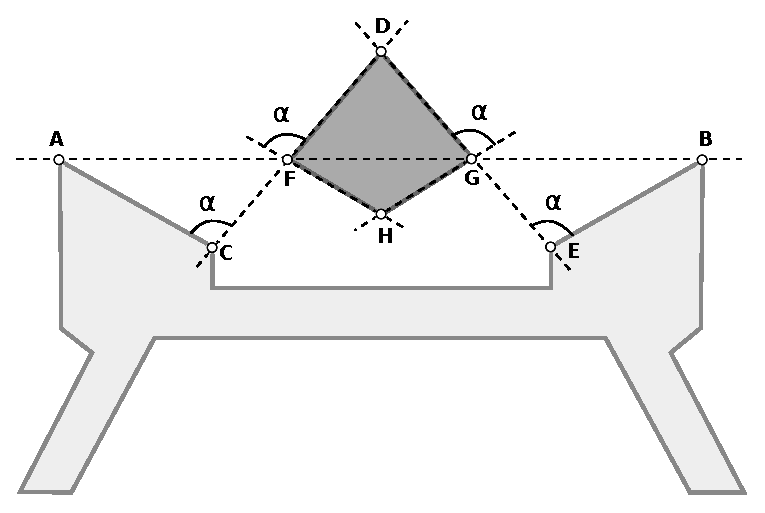
\includegraphics[width=3.25in]{figs/ravelin}
  \caption{Star fortress: Ravelins geometry. Points $F$ and $G$ are calculated intersecting the segment $\overline{AB}$ with segments $\overline{CD}$ and $\overline{ED}$. 
The latter ones are the respective bastion flanks $\overline{AC}$ and $\overline{BE}$ at an user defined angle, close to perpendicular.
Finally, from points $F$ and $G$, two segments, parallel to the bastion flanks, are intersected to get the point $H$.
}
  \label{fig:ravelin}
\end{figure}


\begin{figure}[h]
  \centering
  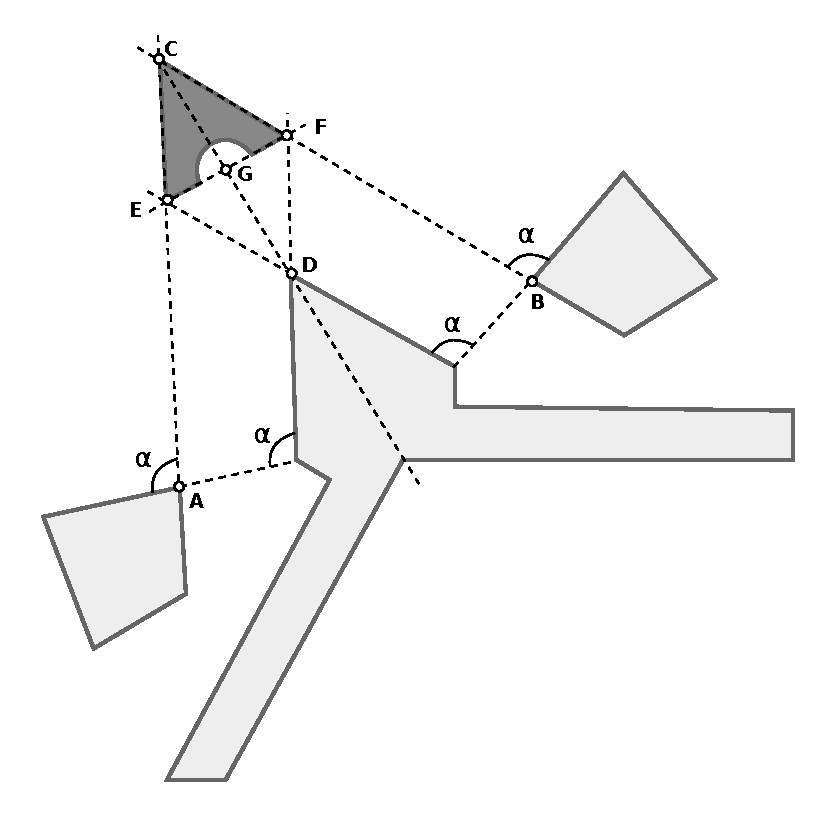
\includegraphics[width=3.25in]{figs/halfmoon}
  \caption{Star fortress: Halfmoon (or Lunettes) geometry. From the rear ravelin flanks, two vectors are traced parallel to the bastion flanks to get the point $C$.
Then, the bastion flanks are extended and intersected with the segments $\overline{AC}$ and $\overline{BC}$ to get the points $E$ and $G$, used both to construct the rear lunette flank.
Finally, the bastion axis is intersected with segment $\overline{EG}$ and a half circle with an user defined radius is constructed on the back. }
  \label{fig:halfmoon}
\end{figure}



\begin{figure}[!h]
  \centering
  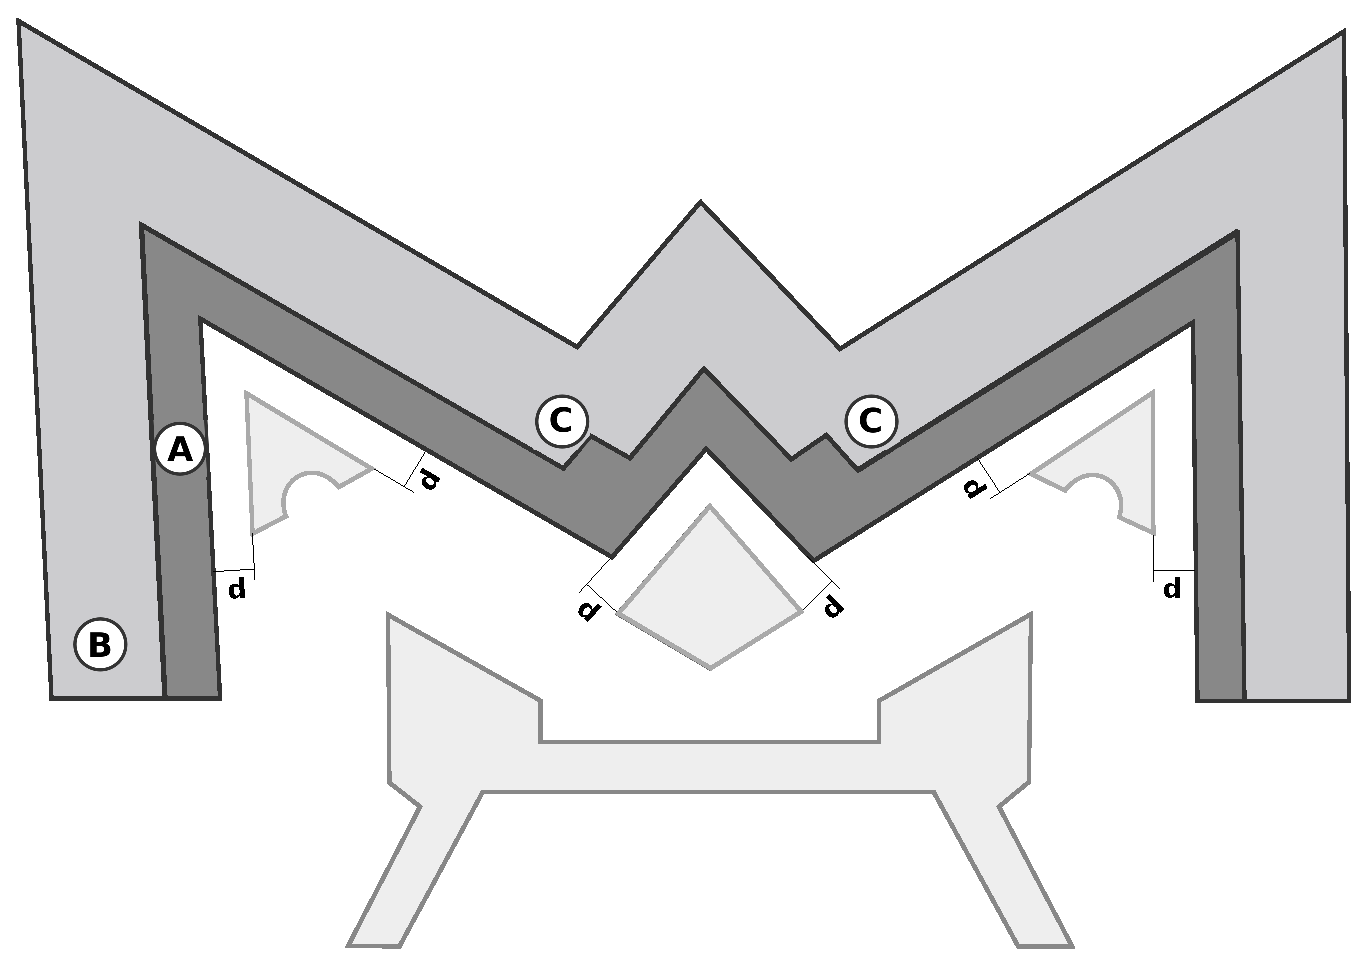
\includegraphics[width=3.25in]{figs/covertway}
  \caption{Star fortress: Covert way, composed by the curtain wall (A), the glacis (B) and the places of arms (C). }
  \label{fig:covertway}
\end{figure}




\newpage

\subsection{Battlefield}
\label{sec:settingsbattlefield}

The battlefield section defines the 2D plan view battlefield sizes and the trenches settings.
The trenches are created automatically and randomly.
The battlefield must be a square.

\begin{tabularx}{0.48\textwidth}{ |l|X| }
\hline 
\textbf{Parameter} & \textbf{Description} \\[0.15cm]
 \hline
 \texttt{size} & Battlefield side length \\
 \hline
 \texttt{GroundCell} & Battlefield cell definition. Many of its parameters are applied to all cells. The API allows to define other values for specific cells. The parameters are: \\
 & \quad\texttt{Size}: Cell side length. \\
 & \quad\texttt{Height}: Cells height. Currently not used. \\
 & \quad\texttt{DefenseIncrease}: Defense value to add at troops deployed on any cell. \\
 & \quad\texttt{MovementPenalty}: Penalty movement applied to battalion movement on the battlefield. It is a percentage that is multiplied by the battalion speed factor. 1.0 means no penalty. \\
 \hline
 \texttt{Trench} & Trenches parameters. There are six parameters: \\
 & \quad\texttt{DefenseIncrease}: Defense value to add at troops deployed on any trench.\\
 & \quad\texttt{MovementPenalty}: Penalty movement for troops on any trench.\\
 & \quad\texttt{ShowOutline}: Set to \texttt{True} if trench outline display is required. For huge battlefields is recommended \texttt{False} value. \\
 & \quad\texttt{RandomDeployment}: Percentage of trenches density along all battlefield. 1 means all cells become trenches. \\
 & \quad\texttt{RandomDeploymentConsecutive}: Trenches size percentage. It defines the probability to get a trench sequence. \\
 & \quad\texttt{RandomDeploymentMaxTries}: Maximum number of tries to get a consecutive trench. Used basically to avoid infinite loops if \textit{RandomDeploymentConsecutive} is closer to 1. \\
 \hline 
 \texttt{River} & Defines the river settings:\\
 & \quad\texttt{PenaltyMovement}: Penalty movement for units through a river (like moats penalty).\\
 \hline
\end{tabularx} 




\subsection{Armies}
\label{sec:settingsarmy}

This section covers the settings for both armies, defenders and attackers.
There are specific settings for each kind of battalion: Infantry, Archers, Cannons, Siege Towers and Throwers (see related sections).
For each kind of battalion, some parameters are common, such are defense or attack values.
The values are not scaled or in any metric, and must be related between the different kind of battalions.
Also, these parameters must be related with the other game elements, such are battlefield (speed, by example) and castle construction elements (tile resistance, by example).
Some of these values are not used in some kind of battalion, but they are specified just to keep the format and standard battle unit definition.


\begin{tabularx}{0.48\textwidth}{ |l|X| }
\hline 
\textbf{Parameter} & \textbf{Description} \\[0.15cm]
 \hline
 \texttt{ShowLabels} & Set to \texttt{True} to display the battalions labels. Usefull for debug purposes.\\
 \hline
\end{tabularx}  
 
\begin{tabularx}{0.48\textwidth}{ |l|X| }
\hline 
\textbf{Parameter} & \textbf{Description} \\[0.15cm]
 \hline
 \texttt{ShowOutline} & Set to \texttt{False} to hide the battalion outline. It is recommended for huge battlefields, where the outline color could overlap the battalion color. \\
 \hline
 \texttt{HumanFieldOfView} & Field of view used for aiming an objective. Used by archers and cannons. \\
 \hline
 \texttt{Infantry} & See Section \ref{sec:settingsinfantry}. \\
 \hline
 \texttt{Archers} & See Section \ref{sec:settingsarchers}. \\
 \hline
 \texttt{Cannons} & See Section \ref{sec:settingscannons}. \\
 \hline
 \texttt{SiegeTowers} & See Section \ref{sec:settingssiegetowers}. \\
 \hline
 \texttt{Throwers} & See Section \ref{sec:settingsthrowers}. \\
 \hline
\end{tabularx} 







\subsubsection{Infantry}
\label{sec:settingsinfantry}

The infantry only plays on the battlefield for the attackers army. Their goal is to advance to the castle and to climb any wall. 
Therefore, the attack parameters are not considered.

\begin{tabularx}{0.48\textwidth}{ |X|X| }
\hline 
\textbf{Parameter} & \textbf{Description} \\[0.15cm]
 \hline
 \texttt{Defense} & Defense value, compared to the attack value. Should be low. \\
 \hline
 \texttt{Attack} & Attack value, compared to the defense value. Infantry units do not attack, so the parameter is not considered.\\
 \hline
 \texttt{Speed} & Movement speed, in distance per turn/step. By example, if battlefield cell size is 10 and speed is 10, the infantry battalions will move to the next cell each turn. \\
 & \qquad \textit{NOTE: Currently a battalion cannot move faster than one cell per turn.} \\
 \hline 
 \texttt{Reload} & Reload time. Not used. \\
 \hline 
 \texttt{Accuracy} & Accuracy shoting. Not used. \\
 \hline 
 \texttt{Distance} & Shooting maximum distance. Not used.\\
 \hline 
 \texttt{Bounding} & Soldier bounding size. Used to know how many soldiers can fit into a battalion that is deployed on a cell. The parameters are \texttt{Length}, \texttt{Width} and \texttt{Height}. \\
 \hline 
 \texttt{ClimbSpeed} & Climbing speed. \\
 \hline 
 \texttt{Stationary} & \texttt{True} if unit cannot move. For infantry it must be \texttt{False}. \\
 \hline 
 \texttt{MovementPriority} & Prority value to decide what unit to move when two of them collide into the same battlefield cell. A battalion with higer value will swap current battalion position by its position. Minimum value: 0. \\
 \hline 
\end{tabularx} 
 
 
\begin{tabularx}{0.48\textwidth}{ |X|X| }
\hline 
 \texttt{MovementPriority WaitingClimbing} & This priority value overrides \texttt{MovementPriority} when the battalion is climbing. The value should be high, so nobody can move the battalion when it is climbing, even siege towers. \\
 \hline 
 \texttt{RubbleClimbSpeed} & Movement speed when infantry moves over wall rubble. \\
 \hline
 \texttt{SearchRadius GoToRumble} & When the infantry is in front of a wall, it decides to climb it on the nearest position or search for any accumulated rubble. This value is the radius search. \\
 \hline
\end{tabularx} 
 
 



\subsubsection{Archers}
\label{sec:settingsarchers}

The archers are the representation of the soldiers who can shoot, either arrows or bullets.
The archers can be deployed on the battlefield as attackers, or on the castle as defenders. 
The battlefield archers can move to reach a good aiming position, and have not any aiming angle restriction.
The castle archers do not move of their position, and inherits the aiming angle restrictions from the castle element where they are deployed.
Therefore, the movement parameters are only applied to the battlefield archers.


\begin{tabularx}{0.48\textwidth}{ |X|X| }
\hline 
\textbf{Parameter} & \textbf{Description} \\[0.15cm]
 \hline
 \texttt{Defense} & Defense value, compared to the attack value. Should be low. \\
 \hline
 \texttt{Attack} & Attack value, compared to the defense value. \\
 \hline
 \texttt{Speed} & Movement speed, in distance per turn/step. \\
 \hline 
 \texttt{Reload} & Reload time. Number of turns/steps to wait until the archer can shoot again. \\
 \hline 
 \texttt{Accuracy} & Accuracy shoot factor, in range [0-100]\% (see Figure \ref{fig:shooting}). \\
 \hline 
 \texttt{Distance} & Shooting maximum distance (see Figure \ref{fig:shooting}).\\
 \hline 
 \texttt{Bounding} & Soldier bounding size. Used to know how many soldiers can fit into a battalion that is deployed on a cell. The parameters are \texttt{Length}, \texttt{Width} and \texttt{Height}. \\
 \hline 
 \texttt{Stationary} & \texttt{True} if unit cannot move. Archers are stationary by nature (except when they move to reach a good aiming position). It must be \texttt{True} in any case. \\
 \hline 
 \texttt{MovementPriority} & Prority value to decide what unit to move when two of them collide into the same battlefield cell. A battalion with higer value will swap current battalion position by its position. Minimum value: 0. \\
 \hline 
\end{tabularx}  
 
\begin{tabularx}{0.48\textwidth}{ |l|X| }
\hline 
\textbf{Parameter} & \textbf{Description} \\[0.15cm]
 \hline
 \texttt{DefenseShoot DoubleCheck} & See below. \\
 \hline
 \texttt{ShootsToStay} & Percentage [0,1]\% of shoots in attack range performed by an archers battalion to decide to stay in its place or to move to a better one. 0 means an absolutely stopped archer, althought it will cannot aim to any target. This parameter is usefull to control the relationship between the archer goal about be covered by a trench, and the archer goal to shoot the closest target. Applied only to the battlefield archers. \\
 \hline
 \texttt{SearchRadius} & \\
 \texttt{Trench} & Search distance to looking for a trench where to be covered from castle shoots. Applied only to the battlefield archers. \\
 \hline
 \texttt{Defenders} & \\
 \texttt{MarginSpace} & Minimum distance between each defender archer in walls or towers. Optional. 0 by default.\\
 \hline 
\end{tabularx} 

When an archer or cannon search for the best target to shoot, it uses the battlefield center position as a fast reference. 
On of the considered parameters is the visibility to the target.
After the cell with the target is selected, a random position inside cell is choosen.
If \texttt{DefenseShootDoubleCheck} parameter is \texttt{True}, the algorithm checks again for the visibility to the new point.
The visibility checking is computionally expensive. 
If the battlefield cells are enough small, it would be good enough setting this flag to \texttt{False}.

 \begin{figure}[ht]
  \centering
  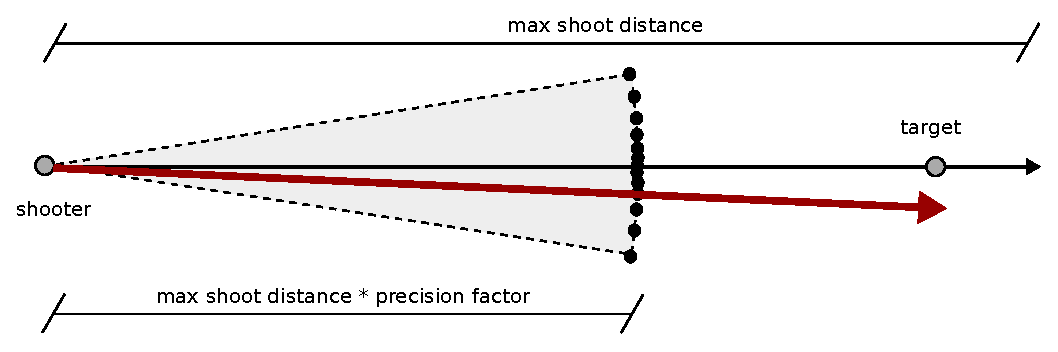
\includegraphics[width=3.25in]{figs/shooting}
  \caption{Shooting method using the precision factor over the maximum shoot distance.}
  \label{fig:shooting}
\end{figure}

\subsubsection{Cannons}
\label{sec:settingscannons}

The cannons are the representation of the artillery.
They cannot move, so the movement parameters are not used.
The soldiers who control the artillery are not considered.



\begin{tabularx}{0.48\textwidth}{ |X|X| }
\hline 
\textbf{Parameter} & \textbf{Description} \\[0.15cm]
 \hline
 \texttt{Defense} & Defense value, compared to the attack value. The cannons should have a high defense value. \\
 \hline
 \texttt{Attack} & Attack value, compared to the defense value. \\
 \hline
 \texttt{Speed} & Movement speed. It should be 0. \\
 \hline 
 \texttt{Reload} & Reload time. Number of turns/steps to wait until the cannon can shoot again. \\
 \hline 
 \texttt{Accuracy} & Accuracy shoot factor, in range [0-100]\% \\
 \hline 
 \texttt{Distance} & Shooting maximum distance.\\
 \hline 
 \texttt{Bounding} & Cannon bounding size. Usually a cannon is enough big to fit only one in one cell. Be aware to set a size less than battalion cell or castle cell sizes. The parameters are \texttt{Length}, \texttt{Width} and \texttt{Height}. \\
 \hline 
 \texttt{Stationary} & A cannon cannot move. It must be \texttt{True}. \\
 \hline 
 \texttt{MovementPriority} & Nothing can move a cannon, so the parameter value should be the larger one. \\
 \hline 
 \texttt{DefenseShoot} & \\
 \texttt{DoubleCheck} & See Section \ref{sec:settingsarchers}. \\
 \hline
 \texttt{ShootAngle} & Angular shooting bounds. The parameters are: \\
 & \quad\texttt{H}: 2D plain view angle (degrees) around the main attack vector. The main vector is the vector from the cannon and target positions.\\
 & \quad\texttt{V}: Vertical angles (in height), from bottom to main attack vector, and from this vector to top. \\
 & \\
 \hline
 \texttt{BallRadius} & Approximated cannon ball radius. It is used when a castle cannon shoots against a battlefield battalion. The ball size is used to estimate the number of killed soldiers. \\
 \hline
 \texttt{DefaultPlacement} & \\
 \texttt{Distance} & Percentage [0,1]\% of the shoot distance used as guide to place the cannons from walls. Low values means best shoots (closer to walls), but less defense condition. \\
 \hline
\end{tabularx} 





\subsubsection{Siege towers}
\label{sec:settingssiegetowers}

The siege tower action starts by its construction. 
At the same time, an infantry unit is selected to cover the castle moat and allow the advance of the structure.
This infantry unit is named \texttt{Turtle}, it can receive shoots from the castle, like another battalion, and it is protected with an effective defense method.
The siege tower has different levels. 
In each level there are archers deployed automatically. 
The number of levels depend on the height of the castle walls, and are selected automatically.


\begin{tabularx}{0.48\textwidth}{ |X|X| }
\hline 
\textbf{Parameter} & \textbf{Description} \\[0.15cm]
 \hline
 \texttt{Defense} & Defense value. \\
 \hline
 \texttt{Attack} & Attack value. It shold be the same value than archers attack parameter. The algorithm multiplies it by the number of internal archers, that is unknown until the siege tower is constructed. \\
 \hline
 \texttt{Speed} & Movement speed. It should be slow. \\
 \hline 
 \texttt{Reload} & Reload time. It should be the same thant the archers reload time parameter. \\
 \hline 
 \texttt{Accuracy} & Accuracy shoot factor, in range [0-100]\%.  It should be the same thant the archers accuracy parameter. \\
 \hline 
 \texttt{Distance} & Shooting maximum distance.  It should be the same thant the archers distance parameter\\
 \hline 
 \texttt{Bounding} & Bounding size. The parameters are \texttt{Length}, \texttt{Width} and \texttt{Height}. The height parameter is not considered, so it is unknonw until the siege tower is constructed.\\
 \hline 
 \texttt{Stationary} & It must be \texttt{False}. \\
 \hline 
 \texttt{Movement} & \\
 \texttt{Priority} & It should has more priority than archers or infantry, but less than cannons. Therefore, a cannon cannot be on the siege tower path to the selected castle wall. \\
 \hline
 \texttt{LevelHeight} & Height for each siege tower level. It should be enough to fit the archers height. The number of siege tower levels is calculated automatically from this height and the castle wall height. \\
 \hline
 \texttt{Construction} & \\
  \texttt{TimePerLevel} & Time spent for the construction of each siege tower level. \\
 \hline
 \texttt{TurtleDefense} & Increased defense to the turtle battalion. \\
 \hline
 \texttt{CoverMoatSpeed} & Spent time to cover one moat cell by the turtle. It should be less than 1. \\
 \hline 
\end{tabularx}





\subsubsection{Throwers}
\label{sec:settingsthrowers}

The throwers are special units created from the closer archers on the castle walls when the attackers start to climb.
The throwers throw dissuasive material to the climbers.
When there are no more climbers, the throwers are dissolved, becoming again normal archers.

\begin{tabularx}{0.48\textwidth}{ |X|X| }
\hline 
\textbf{Parameter} & \textbf{Description} \\[0.15cm]
 \hline
 \texttt{Defense} & Defense value. It should be the same than archers. \\
 \hline
 \texttt{Attack} & Attack value. The damage is applied by distance. The applied damage is the attack divided by the distance per throwers \texttt{Distance} parameter value. \\
 \hline
 \texttt{Speed} & Movement speed. The throwers do not move. \\
 \hline 
 \texttt{Reload} & Reload time. This value will be divided by the battalion size. So, more units on the battalion, less reload time. \\
 \hline 
 \texttt{Accuracy} & Accuracy shoot factor, in range [0-100]\%.  It should be high, so it is easy to shoot a set of soldiers climbing in height. \\
 \hline 
 \texttt{Distance} & Distance attenuation (see \texttt{Attack} value). Greater value means more attenuation. \\
 \hline 
 \texttt{Bounding} & Bounding size. The parameters are \texttt{Length}, \texttt{Width} and \texttt{Height}. The height should be the same than the archers. The length and width are not used, so they are calculated when the thrower battalion is created.\\
 \hline 
 \texttt{Stationary} & It must be \texttt{True}. \\
 \hline 
 \texttt{Movement} & \\
 \texttt{Priority} & Not used. \\
 \hline
 \texttt{Batttalion} & \\
 \texttt{MaxSize} & Maximum number of archers in the battalion. If there are not any closer archer, the battalion is created with less archers. \\
 \hline
\end{tabularx}








\subsection{City Evolution}
\label{sec:settingscity}

The next table shows the parameters to control the city evolution simulation mode. 
See Section \ref{sec:cityevolutions} for the other non-global parameters.


\begin{tabularx}{0.48\textwidth}{ |X|X| }
\hline 
\textbf{Parameter} & \textbf{Description} \\[0.15cm]
 \hline
 \texttt{EvolutionSpeed} & Default simulation speed. Minimum 1, the faster mode. \\
 \hline
 \texttt{YearsPerStep} & Spent years for each turn/step.\\
 \hline
 \texttt{MinWallLength} & Minimum wall length when a new curtain wall is created. \\
 \hline
 \texttt{MaxWallLength} & Maximum wall length when a new curtain wall is created. \\
 \hline
\end{tabularx}  
 
\begin{tabularx}{0.48\textwidth}{ |l|X| }
\hline 
\textbf{Parameter} & \textbf{Description} \\[0.15cm]
 \hline
 \texttt{MatchVertices} & \\
 \texttt{Distance} &  Margin distance to match vertices between two castles in an union operation. Small values means close vertices, therefore close towers. 
 Great values means less close vertices, but some walls could disappear.\\
 \hline
 \texttt{WaitBattle} & This is the time that the system has to spend before check if a battle has finished. This is an issue related with the GUI and threads system, where a manual checking on the thread ending is mandatory. Small values mean many checkings, but large values mean the system could spent too much after a battle end. A value between 1 and 200 should be enough, althought it depends on the used hardware. \\
 \hline
 \texttt{DisplayOldTownGrid} & Displays the inner castle grid. Only for debug purposes. \\
 \hline
 \texttt{Houses} & See below.\\
 \hline
\end{tabularx}


Each house is represented as a small square deployed outside the castle curtain wall. 
The deployment is automatic, using a cosinus random distribution to get a simple urban evolution simulation.
The houses can intersect between them.
The houses creation are controlled by next parameters:

\begin{tabularx}{0.48\textwidth}{ |X|X| }
\hline 
\textbf{Parameter} & \textbf{Description} \\[0.15cm]
 \hline
  \texttt{Size} & Side length of the square that represents a house.\\
 \hline
 \texttt{DistanceWall} & Distance from the curtain wall to deploy the first houses. \\
 \hline
 \texttt{MinDistanceBetween} & Minimum distance between houses. This is only an orientative value, so the minimum distance cannot be controlled due the random deployment (none rejection sampling is used due performance reasons). Try different values and combine them with the maximum distance to get different results. \\
 \hline 
 \texttt{MaxDistanceBetween} & Maximum distance between houses.  \\
 \hline
 \texttt{PlacementFuzzy} & Factor value to apply some jittering to the houses deployment to avoid the patterns that can produce the algorithm. Minimum 1. Larger values means wider and longer radial spaces between houses (them could be considered as some kind of streets). \\
 \hline
\end{tabularx}  
 
\begin{tabularx}{0.48\textwidth}{ |l|X| }
\hline 
\textbf{Parameter} & \textbf{Description} \\[0.15cm]
 \hline
 \texttt{CreationPerYear} & Houses created each year. \\
 \hline
 \texttt{PreferenceFactor} & Priority percentage [0,1]\% on the selection of the older houses to construct new ones aside. Large values could produce an elongate city shape.\\
 \hline
\end{tabularx}




\subsection{Game}
\label{sec:settingsgame}

On the next table there are some paramaters related to the game display:



\begin{tabularx}{0.48\textwidth}{ |X|X| }
\hline 
 \texttt{speed} & Game speed. Minimum 1 (faster). \\
 \hline
 \texttt{WindowHeight} & Window height. Due UI issues, windows and viewports have to be squared. \\
 \hline
 \texttt{WindowWidth} & Window width. \\
 \hline
 \texttt{ViewportHeight} & Viewport height. \\
 \hline
 \texttt{ViewportWidth} & Viewport width. \\
 \hline 
 \texttt{HeightViewHeight} & Height of wall height views. \\
 \hline
 \texttt{HeightViewWidth} & Width of wall width views. \\
 \hline
 \texttt{ShowGrid} & Displays a battlefield grid. Not recommended for huge battlefields. \\
 \hline
\end{tabularx}


















 
\end{document}
